
    % latexmk -pdflatex='lualatex' -pdf FontExhibition.tex
    \documentclass[parskip,landscape,letter]{scrartcl}
    \usepackage{fontspec}
    \usepackage[margin=10mm,left=30mm]{geometry}
    \usepackage{tikz}
    \usetikzlibrary{matrix}
    \usepackage{pifont}
    \usepackage{graphicx}
    \usepackage{diagram}
    \usepackage{setspace}

    \begin{document}
    \setmainfont[Extension={.ttf},ItalicFont={DejaVuSerif-Italic}]{FreeSerif}
    
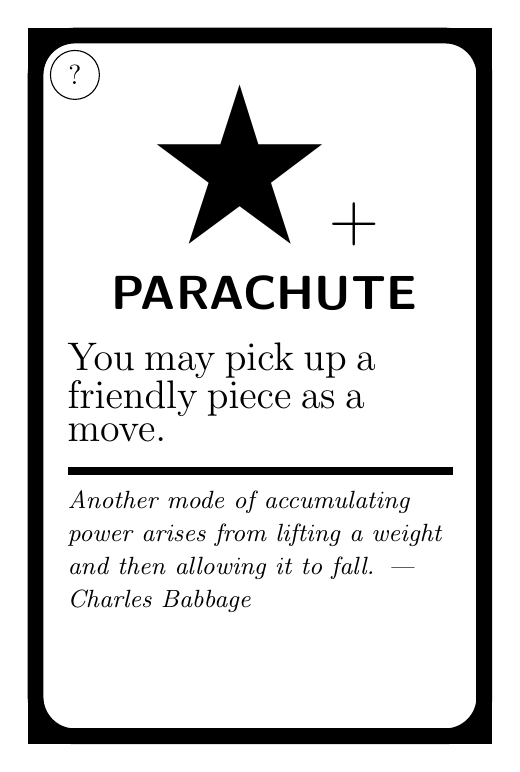
\begin{tikzpicture}
    \pgfmathsetmacro{\cardroundingradius}{5mm}
    \pgfmathsetmacro{\striproundingradius}{3mm}
    % \pgfmathsetmacro{\cardwidth}{5.9}
    % \pgfmathsetmacro{\cardheight}{9.2}
    \pgfmathsetmacro{\cardwidth}{5.7}
    \pgfmathsetmacro{\cardheight}{8.9}
    \pgfmathsetmacro{\stripwidth}{1.2}
    \pgfmathsetmacro{\strippadding}{0.1}
    \pgfmathsetmacro{\textpadding}{0.3}
    \pgfmathsetmacro{\ruleheight}{0.1}
    \providecommand{\stripfontsize}{\Huge}
    \providecommand{\captionfontsize}{\LARGE}
    \providecommand{\textfontsize}{\Large}
    \providecommand{\quotefontsize}{\small}
    \draw[line width=2mm,rounded corners=\cardroundingradius] (0,0) rectangle (\cardwidth,\cardheight);
    \draw[line width=2mm] (0,0) rectangle (\cardwidth,\cardheight);
    \node[text width=(\cardwidth-\strippadding-2*\textpadding)*1cm,below right,inner sep=0] at (\strippadding+\textpadding,\cardheight-\textpadding) 
    { 
    \begin{center} {\fontsize{80pt}{60pt}\selectfont \ding{72}+}\\\end{center}
\begin{center}
    {\captionfontsize \textsf{\textbf{PARACHUTE}}}\end{center}
        {\textfontsize You may pick up a friendly piece as a move.}\\
        \tikz{\fill (0,0) rectangle (\cardwidth-2*\strippadding-2*\textpadding,\ruleheight);}\\
        {\quotefontsize \textit{Another mode of accumulating power arises from lifting a weight and then allowing it to fall. ---Charles Babbage}}\\[-2\baselineskip]
    };
    \node[circle,draw,text=black](c) at (.5,\cardheight-.5){?};
    \end{tikzpicture}%
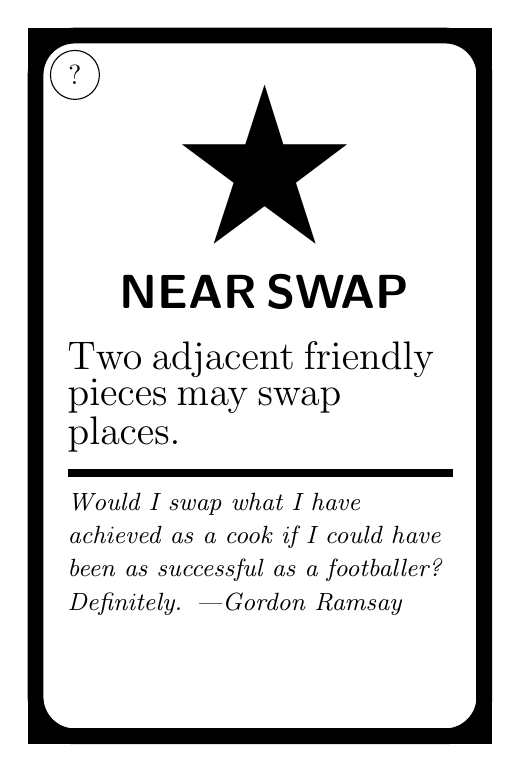
\begin{tikzpicture}
    \pgfmathsetmacro{\cardroundingradius}{5mm}
    \pgfmathsetmacro{\striproundingradius}{3mm}
    % \pgfmathsetmacro{\cardwidth}{5.9}
    % \pgfmathsetmacro{\cardheight}{9.2}
    \pgfmathsetmacro{\cardwidth}{5.7}
    \pgfmathsetmacro{\cardheight}{8.9}
    \pgfmathsetmacro{\stripwidth}{1.2}
    \pgfmathsetmacro{\strippadding}{0.1}
    \pgfmathsetmacro{\textpadding}{0.3}
    \pgfmathsetmacro{\ruleheight}{0.1}
    \providecommand{\stripfontsize}{\Huge}
    \providecommand{\captionfontsize}{\LARGE}
    \providecommand{\textfontsize}{\Large}
    \providecommand{\quotefontsize}{\small}
    \draw[line width=2mm,rounded corners=\cardroundingradius] (0,0) rectangle (\cardwidth,\cardheight);
    \draw[line width=2mm] (0,0) rectangle (\cardwidth,\cardheight);
    \node[text width=(\cardwidth-\strippadding-2*\textpadding)*1cm,below right,inner sep=0] at (\strippadding+\textpadding,\cardheight-\textpadding) 
    { 
    \begin{center} {\fontsize{80pt}{60pt}\selectfont \ding{72}}\\\end{center}
\begin{center}
    {\captionfontsize \textsf{\textbf{NEAR SWAP}}}\end{center}
        {\textfontsize Two adjacent friendly pieces may swap places.}\\
        \tikz{\fill (0,0) rectangle (\cardwidth-2*\strippadding-2*\textpadding,\ruleheight);}\\
        {\quotefontsize \textit{Would I swap what I have achieved as a cook if I could have been as successful as a footballer? Definitely. ---Gordon Ramsay}}\\[-2\baselineskip]
    };
    \node[circle,draw,text=black](c) at (.5,\cardheight-.5){?};
    \end{tikzpicture}%
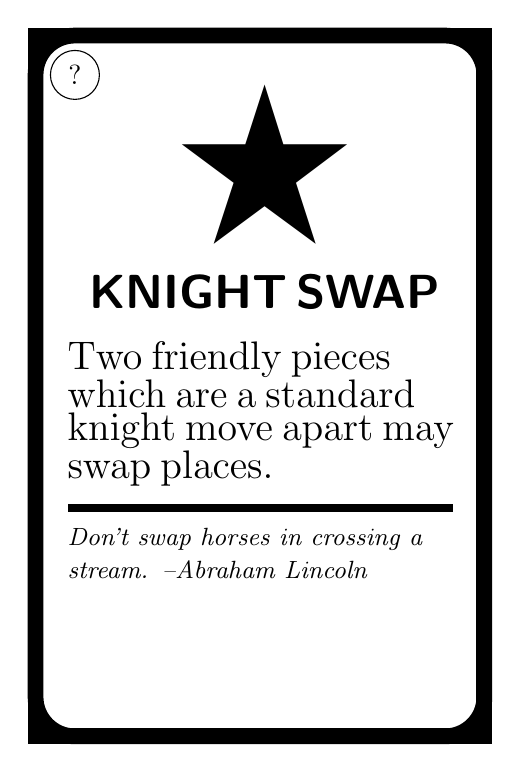
\begin{tikzpicture}
    \pgfmathsetmacro{\cardroundingradius}{5mm}
    \pgfmathsetmacro{\striproundingradius}{3mm}
    % \pgfmathsetmacro{\cardwidth}{5.9}
    % \pgfmathsetmacro{\cardheight}{9.2}
    \pgfmathsetmacro{\cardwidth}{5.7}
    \pgfmathsetmacro{\cardheight}{8.9}
    \pgfmathsetmacro{\stripwidth}{1.2}
    \pgfmathsetmacro{\strippadding}{0.1}
    \pgfmathsetmacro{\textpadding}{0.3}
    \pgfmathsetmacro{\ruleheight}{0.1}
    \providecommand{\stripfontsize}{\Huge}
    \providecommand{\captionfontsize}{\LARGE}
    \providecommand{\textfontsize}{\Large}
    \providecommand{\quotefontsize}{\small}
    \draw[line width=2mm,rounded corners=\cardroundingradius] (0,0) rectangle (\cardwidth,\cardheight);
    \draw[line width=2mm] (0,0) rectangle (\cardwidth,\cardheight);
    \node[text width=(\cardwidth-\strippadding-2*\textpadding)*1cm,below right,inner sep=0] at (\strippadding+\textpadding,\cardheight-\textpadding) 
    { 
    \begin{center} {\fontsize{80pt}{60pt}\selectfont \ding{72}}\\\end{center}
\begin{center}
    {\captionfontsize \textsf{\textbf{KNIGHT SWAP}}}\end{center}
        {\textfontsize Two friendly pieces which are a standard knight move apart may swap places.}\\
        \tikz{\fill (0,0) rectangle (\cardwidth-2*\strippadding-2*\textpadding,\ruleheight);}\\
        {\quotefontsize \textit{Don't swap horses in crossing a stream. --Abraham Lincoln}}\\[-2\baselineskip]
    };
    \node[circle,draw,text=black](c) at (.5,\cardheight-.5){?};
    \end{tikzpicture}%
\begin{tikzpicture}
    \pgfmathsetmacro{\cardroundingradius}{5mm}
    \pgfmathsetmacro{\striproundingradius}{3mm}
    % \pgfmathsetmacro{\cardwidth}{5.9}
    % \pgfmathsetmacro{\cardheight}{9.2}
    \pgfmathsetmacro{\cardwidth}{5.7}
    \pgfmathsetmacro{\cardheight}{8.9}
    \pgfmathsetmacro{\stripwidth}{1.2}
    \pgfmathsetmacro{\strippadding}{0.1}
    \pgfmathsetmacro{\textpadding}{0.3}
    \pgfmathsetmacro{\ruleheight}{0.1}
    \providecommand{\stripfontsize}{\Huge}
    \providecommand{\captionfontsize}{\LARGE}
    \providecommand{\textfontsize}{\Large}
    \providecommand{\quotefontsize}{\small}
    \draw[line width=2mm,rounded corners=\cardroundingradius] (0,0) rectangle (\cardwidth,\cardheight);
    \draw[line width=2mm] (0,0) rectangle (\cardwidth,\cardheight);
    \node[text width=(\cardwidth-\strippadding-2*\textpadding)*1cm,below right,inner sep=0] at (\strippadding+\textpadding,\cardheight-\textpadding) 
    { 
    \begin{center} {\fontsize{80pt}{60pt}\selectfont ♖}\\\end{center}
\begin{center}
    {\captionfontsize \textsf{\textbf{SIEGE TOWER}}}\end{center}
        {\textfontsize \small A piece may move legally to where there is a rook. It goes on top making a combined piece. The combination acts as the bottom rook. The piece on top can move off as a normal action. Stacks are ok. Multi-color is ok.}\\
        \tikz{\fill (0,0) rectangle (\cardwidth-2*\strippadding-2*\textpadding,\ruleheight);}\\
        {\quotefontsize \textit{A siege is an act of war. ---Noam Chomsky}}\\[-2\baselineskip]
    };
    \node[circle,draw,text=black](c) at (.5,\cardheight-.5){?};
    \end{tikzpicture}%
\\[-\lineskip]
\begin{tikzpicture}
    \pgfmathsetmacro{\cardroundingradius}{5mm}
    \pgfmathsetmacro{\striproundingradius}{3mm}
    % \pgfmathsetmacro{\cardwidth}{5.9}
    % \pgfmathsetmacro{\cardheight}{9.2}
    \pgfmathsetmacro{\cardwidth}{5.7}
    \pgfmathsetmacro{\cardheight}{8.9}
    \pgfmathsetmacro{\stripwidth}{1.2}
    \pgfmathsetmacro{\strippadding}{0.1}
    \pgfmathsetmacro{\textpadding}{0.3}
    \pgfmathsetmacro{\ruleheight}{0.1}
    \providecommand{\stripfontsize}{\Huge}
    \providecommand{\captionfontsize}{\LARGE}
    \providecommand{\textfontsize}{\Large}
    \providecommand{\quotefontsize}{\small}
    \draw[line width=2mm,rounded corners=\cardroundingradius] (0,0) rectangle (\cardwidth,\cardheight);
    \draw[line width=2mm] (0,0) rectangle (\cardwidth,\cardheight);
    \node[text width=(\cardwidth-\strippadding-2*\textpadding)*1cm,below right,inner sep=0] at (\strippadding+\textpadding,\cardheight-\textpadding) 
    { 
    \begin{center} {\fontsize{80pt}{60pt}\selectfont ♔}\\\end{center}
\begin{center}
    {\captionfontsize \textsf{\textbf{FAR MIMIC}}}\end{center}
        {\textfontsize Kings act only as any friendly piece which can move to it. No castling.}\\
        \tikz{\fill (0,0) rectangle (\cardwidth-2*\strippadding-2*\textpadding,\ruleheight);}\\
        {\quotefontsize \textit{I've been imitated so well I've heard people copy my mistakes. ---Jimi Hendrix}}\\[-2\baselineskip]
    };
    \node[circle,draw,text=black](c) at (.5,\cardheight-.5){C};
    \end{tikzpicture}%
\begin{tikzpicture}
    \pgfmathsetmacro{\cardroundingradius}{5mm}
    \pgfmathsetmacro{\striproundingradius}{3mm}
    % \pgfmathsetmacro{\cardwidth}{5.9}
    % \pgfmathsetmacro{\cardheight}{9.2}
    \pgfmathsetmacro{\cardwidth}{5.7}
    \pgfmathsetmacro{\cardheight}{8.9}
    \pgfmathsetmacro{\stripwidth}{1.2}
    \pgfmathsetmacro{\strippadding}{0.1}
    \pgfmathsetmacro{\textpadding}{0.3}
    \pgfmathsetmacro{\ruleheight}{0.1}
    \providecommand{\stripfontsize}{\Huge}
    \providecommand{\captionfontsize}{\LARGE}
    \providecommand{\textfontsize}{\Large}
    \providecommand{\quotefontsize}{\small}
    \draw[line width=2mm,rounded corners=\cardroundingradius] (0,0) rectangle (\cardwidth,\cardheight);
    \draw[line width=2mm] (0,0) rectangle (\cardwidth,\cardheight);
    \node[text width=(\cardwidth-\strippadding-2*\textpadding)*1cm,below right,inner sep=0] at (\strippadding+\textpadding,\cardheight-\textpadding) 
    { 
    \begin{center} {\fontsize{80pt}{60pt}\selectfont ♖}\\\end{center}
\begin{center}
    {\captionfontsize \textsf{\textbf{CROWNED CASTLE}}}\end{center}
        {\textfontsize Rooks may also move/take like a King.}\\
        \tikz{\fill (0,0) rectangle (\cardwidth-2*\strippadding-2*\textpadding,\ruleheight);}\\
        {\quotefontsize \textit{In the land of the skunks, he who has half a nose is king. ---Chris Farley}}\\[-2\baselineskip]
    };
    \node[circle,draw,text=black](c) at (.5,\cardheight-.5){I};
    \end{tikzpicture}%
\begin{tikzpicture}
    \pgfmathsetmacro{\cardroundingradius}{5mm}
    \pgfmathsetmacro{\striproundingradius}{3mm}
    % \pgfmathsetmacro{\cardwidth}{5.9}
    % \pgfmathsetmacro{\cardheight}{9.2}
    \pgfmathsetmacro{\cardwidth}{5.7}
    \pgfmathsetmacro{\cardheight}{8.9}
    \pgfmathsetmacro{\stripwidth}{1.2}
    \pgfmathsetmacro{\strippadding}{0.1}
    \pgfmathsetmacro{\textpadding}{0.3}
    \pgfmathsetmacro{\ruleheight}{0.1}
    \providecommand{\stripfontsize}{\Huge}
    \providecommand{\captionfontsize}{\LARGE}
    \providecommand{\textfontsize}{\Large}
    \providecommand{\quotefontsize}{\small}
    \draw[line width=2mm,rounded corners=\cardroundingradius] (0,0) rectangle (\cardwidth,\cardheight);
    \draw[line width=2mm] (0,0) rectangle (\cardwidth,\cardheight);
    \node[text width=(\cardwidth-\strippadding-2*\textpadding)*1cm,below right,inner sep=0] at (\strippadding+\textpadding,\cardheight-\textpadding) 
    { 
    \begin{center} {\fontsize{80pt}{60pt}\selectfont ♗}\\\end{center}
\begin{center}
    {\captionfontsize \textsf{\textbf{CROWNED BISHOP}}}\end{center}
        {\textfontsize Bishops may also move/take like a King.}\\
        \tikz{\fill (0,0) rectangle (\cardwidth-2*\strippadding-2*\textpadding,\ruleheight);}\\
        {\quotefontsize \textit{In the land of the blind the one-eyed man is king. ---Efren Ramirez}}\\[-2\baselineskip]
    };
    \node[circle,draw,text=black](c) at (.5,\cardheight-.5){I};
    \end{tikzpicture}%
\begin{tikzpicture}
    \pgfmathsetmacro{\cardroundingradius}{5mm}
    \pgfmathsetmacro{\striproundingradius}{3mm}
    % \pgfmathsetmacro{\cardwidth}{5.9}
    % \pgfmathsetmacro{\cardheight}{9.2}
    \pgfmathsetmacro{\cardwidth}{5.7}
    \pgfmathsetmacro{\cardheight}{8.9}
    \pgfmathsetmacro{\stripwidth}{1.2}
    \pgfmathsetmacro{\strippadding}{0.1}
    \pgfmathsetmacro{\textpadding}{0.3}
    \pgfmathsetmacro{\ruleheight}{0.1}
    \providecommand{\stripfontsize}{\Huge}
    \providecommand{\captionfontsize}{\LARGE}
    \providecommand{\textfontsize}{\Large}
    \providecommand{\quotefontsize}{\small}
    \draw[line width=2mm,rounded corners=\cardroundingradius] (0,0) rectangle (\cardwidth,\cardheight);
    \draw[line width=2mm] (0,0) rectangle (\cardwidth,\cardheight);
    \node[text width=(\cardwidth-\strippadding-2*\textpadding)*1cm,below right,inner sep=0] at (\strippadding+\textpadding,\cardheight-\textpadding) 
    { 
    \begin{center} {\fontsize{80pt}{60pt}\selectfont ♔}\\\end{center}
\begin{center}
    {\captionfontsize \textsf{\textbf{NEAR MIMIC}}}\end{center}
        {\textfontsize Kings act only as any adjacent friendly piece. No castling.}\\
        \tikz{\fill (0,0) rectangle (\cardwidth-2*\strippadding-2*\textpadding,\ruleheight);}\\
        {\quotefontsize \textit{You can't really copy what I do because I don't do anything. ---David Bailey}}\\[-2\baselineskip]
    };
    \node[circle,draw,text=black](c) at (.5,\cardheight-.5){C};
    \end{tikzpicture}%
\\[-\lineskip]
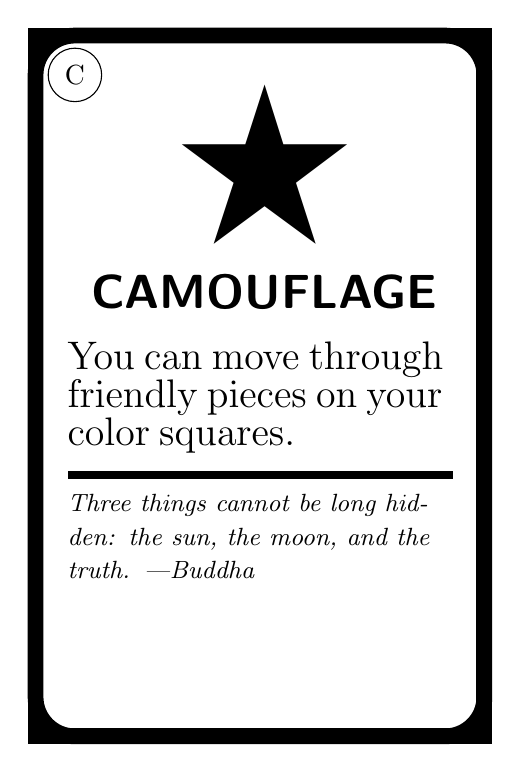
\begin{tikzpicture}
    \pgfmathsetmacro{\cardroundingradius}{5mm}
    \pgfmathsetmacro{\striproundingradius}{3mm}
    % \pgfmathsetmacro{\cardwidth}{5.9}
    % \pgfmathsetmacro{\cardheight}{9.2}
    \pgfmathsetmacro{\cardwidth}{5.7}
    \pgfmathsetmacro{\cardheight}{8.9}
    \pgfmathsetmacro{\stripwidth}{1.2}
    \pgfmathsetmacro{\strippadding}{0.1}
    \pgfmathsetmacro{\textpadding}{0.3}
    \pgfmathsetmacro{\ruleheight}{0.1}
    \providecommand{\stripfontsize}{\Huge}
    \providecommand{\captionfontsize}{\LARGE}
    \providecommand{\textfontsize}{\Large}
    \providecommand{\quotefontsize}{\small}
    \draw[line width=2mm,rounded corners=\cardroundingradius] (0,0) rectangle (\cardwidth,\cardheight);
    \draw[line width=2mm] (0,0) rectangle (\cardwidth,\cardheight);
    \node[text width=(\cardwidth-\strippadding-2*\textpadding)*1cm,below right,inner sep=0] at (\strippadding+\textpadding,\cardheight-\textpadding) 
    { 
    \begin{center} {\fontsize{80pt}{60pt}\selectfont \ding{72}}\\\end{center}
\begin{center}
    {\captionfontsize \textsf{\textbf{CAMOUFLAGE}}}\end{center}
        {\textfontsize You can move through friendly pieces on your color squares.}\\
        \tikz{\fill (0,0) rectangle (\cardwidth-2*\strippadding-2*\textpadding,\ruleheight);}\\
        {\quotefontsize \textit{Three things cannot be long hidden: the sun, the moon, and the truth. ---Buddha}}\\[-2\baselineskip]
    };
    \node[circle,draw,text=black](c) at (.5,\cardheight-.5){C};
    \end{tikzpicture}%
\begin{tikzpicture}
    \pgfmathsetmacro{\cardroundingradius}{5mm}
    \pgfmathsetmacro{\striproundingradius}{3mm}
    % \pgfmathsetmacro{\cardwidth}{5.9}
    % \pgfmathsetmacro{\cardheight}{9.2}
    \pgfmathsetmacro{\cardwidth}{5.7}
    \pgfmathsetmacro{\cardheight}{8.9}
    \pgfmathsetmacro{\stripwidth}{1.2}
    \pgfmathsetmacro{\strippadding}{0.1}
    \pgfmathsetmacro{\textpadding}{0.3}
    \pgfmathsetmacro{\ruleheight}{0.1}
    \providecommand{\stripfontsize}{\Huge}
    \providecommand{\captionfontsize}{\LARGE}
    \providecommand{\textfontsize}{\Large}
    \providecommand{\quotefontsize}{\small}
    \draw[line width=2mm,rounded corners=\cardroundingradius] (0,0) rectangle (\cardwidth,\cardheight);
    \draw[line width=2mm] (0,0) rectangle (\cardwidth,\cardheight);
    \node[text width=(\cardwidth-\strippadding-2*\textpadding)*1cm,below right,inner sep=0] at (\strippadding+\textpadding,\cardheight-\textpadding) 
    { 
    \begin{center} {\fontsize{80pt}{60pt}\selectfont ♘}\\\end{center}
\begin{center}
    {\captionfontsize \textsf{\textbf{KNIGHT+ v1}}}\end{center}
        {\textfontsize Knights may also move/take $[\pm 1, \pm 1]$.}\\
        \tikz{\fill (0,0) rectangle (\cardwidth-2*\strippadding-2*\textpadding,\ruleheight);}\\
        {\quotefontsize \textit{Graphic needed.}}\\[-2\baselineskip]
    };
    \node[circle,draw,text=black](c) at (.5,\cardheight-.5){I};
    \end{tikzpicture}%
\begin{tikzpicture}
    \pgfmathsetmacro{\cardroundingradius}{5mm}
    \pgfmathsetmacro{\striproundingradius}{3mm}
    % \pgfmathsetmacro{\cardwidth}{5.9}
    % \pgfmathsetmacro{\cardheight}{9.2}
    \pgfmathsetmacro{\cardwidth}{5.7}
    \pgfmathsetmacro{\cardheight}{8.9}
    \pgfmathsetmacro{\stripwidth}{1.2}
    \pgfmathsetmacro{\strippadding}{0.1}
    \pgfmathsetmacro{\textpadding}{0.3}
    \pgfmathsetmacro{\ruleheight}{0.1}
    \providecommand{\stripfontsize}{\Huge}
    \providecommand{\captionfontsize}{\LARGE}
    \providecommand{\textfontsize}{\Large}
    \providecommand{\quotefontsize}{\small}
    \draw[line width=2mm,rounded corners=\cardroundingradius] (0,0) rectangle (\cardwidth,\cardheight);
    \draw[line width=2mm] (0,0) rectangle (\cardwidth,\cardheight);
    \node[text width=(\cardwidth-\strippadding-2*\textpadding)*1cm,below right,inner sep=0] at (\strippadding+\textpadding,\cardheight-\textpadding) 
    { 
    \begin{center} {\fontsize{80pt}{60pt}\selectfont ♘}\\\end{center}
\begin{center}
    {\captionfontsize \textsf{\textbf{KNIGHT+ v2}}}\end{center}
        {\textfontsize Knights may also move/take $[\pm 2, \pm 2]$.}\\
        \tikz{\fill (0,0) rectangle (\cardwidth-2*\strippadding-2*\textpadding,\ruleheight);}\\
        {\quotefontsize \textit{Graphic needed.}}\\[-2\baselineskip]
    };
    \node[circle,draw,text=black](c) at (.5,\cardheight-.5){I};
    \end{tikzpicture}%
\begin{tikzpicture}
    \pgfmathsetmacro{\cardroundingradius}{5mm}
    \pgfmathsetmacro{\striproundingradius}{3mm}
    % \pgfmathsetmacro{\cardwidth}{5.9}
    % \pgfmathsetmacro{\cardheight}{9.2}
    \pgfmathsetmacro{\cardwidth}{5.7}
    \pgfmathsetmacro{\cardheight}{8.9}
    \pgfmathsetmacro{\stripwidth}{1.2}
    \pgfmathsetmacro{\strippadding}{0.1}
    \pgfmathsetmacro{\textpadding}{0.3}
    \pgfmathsetmacro{\ruleheight}{0.1}
    \providecommand{\stripfontsize}{\Huge}
    \providecommand{\captionfontsize}{\LARGE}
    \providecommand{\textfontsize}{\Large}
    \providecommand{\quotefontsize}{\small}
    \draw[line width=2mm,rounded corners=\cardroundingradius] (0,0) rectangle (\cardwidth,\cardheight);
    \draw[line width=2mm] (0,0) rectangle (\cardwidth,\cardheight);
    \node[text width=(\cardwidth-\strippadding-2*\textpadding)*1cm,below right,inner sep=0] at (\strippadding+\textpadding,\cardheight-\textpadding) 
    { 
    \begin{center} {\fontsize{80pt}{60pt}\selectfont ♘}\\\end{center}
\begin{center}
    {\captionfontsize \textsf{\textbf{KNIGHT+ v3}}}\end{center}
        {\textfontsize Knights may also move/take one square orthogonally, $[1,0]$ and $[0,1]$.}\\
        \tikz{\fill (0,0) rectangle (\cardwidth-2*\strippadding-2*\textpadding,\ruleheight);}\\
        {\quotefontsize \textit{Graphic needed.}}\\[-2\baselineskip]
    };
    \node[circle,draw,text=black](c) at (.5,\cardheight-.5){I};
    \end{tikzpicture}%
\\[-\lineskip]
\begin{tikzpicture}
    \pgfmathsetmacro{\cardroundingradius}{5mm}
    \pgfmathsetmacro{\striproundingradius}{3mm}
    % \pgfmathsetmacro{\cardwidth}{5.9}
    % \pgfmathsetmacro{\cardheight}{9.2}
    \pgfmathsetmacro{\cardwidth}{5.7}
    \pgfmathsetmacro{\cardheight}{8.9}
    \pgfmathsetmacro{\stripwidth}{1.2}
    \pgfmathsetmacro{\strippadding}{0.1}
    \pgfmathsetmacro{\textpadding}{0.3}
    \pgfmathsetmacro{\ruleheight}{0.1}
    \providecommand{\stripfontsize}{\Huge}
    \providecommand{\captionfontsize}{\LARGE}
    \providecommand{\textfontsize}{\Large}
    \providecommand{\quotefontsize}{\small}
    \draw[line width=2mm,rounded corners=\cardroundingradius] (0,0) rectangle (\cardwidth,\cardheight);
    \draw[line width=2mm] (0,0) rectangle (\cardwidth,\cardheight);
    \node[text width=(\cardwidth-\strippadding-2*\textpadding)*1cm,below right,inner sep=0] at (\strippadding+\textpadding,\cardheight-\textpadding) 
    { 
    \begin{center} {\fontsize{80pt}{60pt}\selectfont ♘}\\\end{center}
\begin{center}
    {\captionfontsize \textsf{\textbf{KNIGHT+ v4}}}\end{center}
        {\textfontsize Knights may also move/take twos square orthogonally, $[2,0]$ and $[0,2]$.}\\
        \tikz{\fill (0,0) rectangle (\cardwidth-2*\strippadding-2*\textpadding,\ruleheight);}\\
        {\quotefontsize \textit{Graphic needed.}}\\[-2\baselineskip]
    };
    \node[circle,draw,text=black](c) at (.5,\cardheight-.5){I};
    \end{tikzpicture}%
\begin{tikzpicture}
    \pgfmathsetmacro{\cardroundingradius}{5mm}
    \pgfmathsetmacro{\striproundingradius}{3mm}
    % \pgfmathsetmacro{\cardwidth}{5.9}
    % \pgfmathsetmacro{\cardheight}{9.2}
    \pgfmathsetmacro{\cardwidth}{5.7}
    \pgfmathsetmacro{\cardheight}{8.9}
    \pgfmathsetmacro{\stripwidth}{1.2}
    \pgfmathsetmacro{\strippadding}{0.1}
    \pgfmathsetmacro{\textpadding}{0.3}
    \pgfmathsetmacro{\ruleheight}{0.1}
    \providecommand{\stripfontsize}{\Huge}
    \providecommand{\captionfontsize}{\LARGE}
    \providecommand{\textfontsize}{\Large}
    \providecommand{\quotefontsize}{\small}
    \draw[line width=2mm,rounded corners=\cardroundingradius] (0,0) rectangle (\cardwidth,\cardheight);
    \draw[line width=2mm] (0,0) rectangle (\cardwidth,\cardheight);
    \node[text width=(\cardwidth-\strippadding-2*\textpadding)*1cm,below right,inner sep=0] at (\strippadding+\textpadding,\cardheight-\textpadding) 
    { 
    \begin{center} {\fontsize{80pt}{60pt}\selectfont ♙+}\\\end{center}
\begin{center}
    {\captionfontsize \textsf{\textbf{PRECOCIOUS PAWNS}}}\end{center}
        {\textfontsize Pawns start advanced one rank. Draw another card.}\\
        \tikz{\fill (0,0) rectangle (\cardwidth-2*\strippadding-2*\textpadding,\ruleheight);}\\
        {\quotefontsize \textit{Precocious was not the same as smart, much less the same as wise, and the perfect opposite of informed. ---Lionel Shriver}}\\[-2\baselineskip]
    };
    \node[circle,draw,text=black](c) at (.5,\cardheight-.5){I};
    \end{tikzpicture}%
\begin{tikzpicture}
    \pgfmathsetmacro{\cardroundingradius}{5mm}
    \pgfmathsetmacro{\striproundingradius}{3mm}
    % \pgfmathsetmacro{\cardwidth}{5.9}
    % \pgfmathsetmacro{\cardheight}{9.2}
    \pgfmathsetmacro{\cardwidth}{5.7}
    \pgfmathsetmacro{\cardheight}{8.9}
    \pgfmathsetmacro{\stripwidth}{1.2}
    \pgfmathsetmacro{\strippadding}{0.1}
    \pgfmathsetmacro{\textpadding}{0.3}
    \pgfmathsetmacro{\ruleheight}{0.1}
    \providecommand{\stripfontsize}{\Huge}
    \providecommand{\captionfontsize}{\LARGE}
    \providecommand{\textfontsize}{\Large}
    \providecommand{\quotefontsize}{\small}
    \draw[line width=2mm,rounded corners=\cardroundingradius] (0,0) rectangle (\cardwidth,\cardheight);
    \draw[line width=2mm] (0,0) rectangle (\cardwidth,\cardheight);
    \node[text width=(\cardwidth-\strippadding-2*\textpadding)*1cm,below right,inner sep=0] at (\strippadding+\textpadding,\cardheight-\textpadding) 
    { 
    \begin{center} {\fontsize{80pt}{60pt}\selectfont ♙}\\\end{center}
\begin{center}
    {\captionfontsize \textsf{\textbf{CHECKERS}}}\end{center}
        {\textfontsize Pawns move and take like checkers.}\\
        \tikz{\fill (0,0) rectangle (\cardwidth-2*\strippadding-2*\textpadding,\ruleheight);}\\
        {\quotefontsize \textit{These guys are playing checkers. I'm out here playing chess. When they figure it out, it's too late. ---Max Holloway}}\\[-2\baselineskip]
    };
    \node[circle,draw,text=black](c) at (.5,\cardheight-.5){C};
    \end{tikzpicture}%
\begin{tikzpicture}
    \pgfmathsetmacro{\cardroundingradius}{5mm}
    \pgfmathsetmacro{\striproundingradius}{3mm}
    % \pgfmathsetmacro{\cardwidth}{5.9}
    % \pgfmathsetmacro{\cardheight}{9.2}
    \pgfmathsetmacro{\cardwidth}{5.7}
    \pgfmathsetmacro{\cardheight}{8.9}
    \pgfmathsetmacro{\stripwidth}{1.2}
    \pgfmathsetmacro{\strippadding}{0.1}
    \pgfmathsetmacro{\textpadding}{0.3}
    \pgfmathsetmacro{\ruleheight}{0.1}
    \providecommand{\stripfontsize}{\Huge}
    \providecommand{\captionfontsize}{\LARGE}
    \providecommand{\textfontsize}{\Large}
    \providecommand{\quotefontsize}{\small}
    \draw[line width=2mm,rounded corners=\cardroundingradius] (0,0) rectangle (\cardwidth,\cardheight);
    \draw[line width=2mm] (0,0) rectangle (\cardwidth,\cardheight);
    \node[text width=(\cardwidth-\strippadding-2*\textpadding)*1cm,below right,inner sep=0] at (\strippadding+\textpadding,\cardheight-\textpadding) 
    { 
    \begin{center} {\fontsize{80pt}{60pt}\selectfont ♗}\\\end{center}
\begin{center}
    {\captionfontsize \textsf{\textbf{BISHOP CHAMELEON}}}\end{center}
        {\textfontsize Bishops move normally, but only attack pieces that attack them. Bishops attack each other normally.}\\
        \tikz{\fill (0,0) rectangle (\cardwidth-2*\strippadding-2*\textpadding,\ruleheight);}\\
        {\quotefontsize \textit{I could spend the rest of my life in copying a chair. ---Alberto Giacometti}}\\[-2\baselineskip]
    };
    \node[circle,draw,text=black](c) at (.5,\cardheight-.5){U};
    \end{tikzpicture}%
\\[-\lineskip]
\begin{tikzpicture}
    \pgfmathsetmacro{\cardroundingradius}{5mm}
    \pgfmathsetmacro{\striproundingradius}{3mm}
    % \pgfmathsetmacro{\cardwidth}{5.9}
    % \pgfmathsetmacro{\cardheight}{9.2}
    \pgfmathsetmacro{\cardwidth}{5.7}
    \pgfmathsetmacro{\cardheight}{8.9}
    \pgfmathsetmacro{\stripwidth}{1.2}
    \pgfmathsetmacro{\strippadding}{0.1}
    \pgfmathsetmacro{\textpadding}{0.3}
    \pgfmathsetmacro{\ruleheight}{0.1}
    \providecommand{\stripfontsize}{\Huge}
    \providecommand{\captionfontsize}{\LARGE}
    \providecommand{\textfontsize}{\Large}
    \providecommand{\quotefontsize}{\small}
    \draw[line width=2mm,rounded corners=\cardroundingradius] (0,0) rectangle (\cardwidth,\cardheight);
    \draw[line width=2mm] (0,0) rectangle (\cardwidth,\cardheight);
    \node[text width=(\cardwidth-\strippadding-2*\textpadding)*1cm,below right,inner sep=0] at (\strippadding+\textpadding,\cardheight-\textpadding) 
    { 
    \begin{center} {\fontsize{80pt}{60pt}\selectfont ♘♗}\\\end{center}
\begin{center}
    {\captionfontsize \textsf{\textbf{BISHOP-KNIGHT SWAP}}}\end{center}
        {\textfontsize Bishops take like Knights. Knights take like Bishops. Movement remains unchanged.}\\
        \tikz{\fill (0,0) rectangle (\cardwidth-2*\strippadding-2*\textpadding,\ruleheight);}\\
        {\quotefontsize \textit{It's time to bait a trap. ---Katie Reus}}\\[-2\baselineskip]
    };
    \node[circle,draw,text=black](c) at (.5,\cardheight-.5){?};
    \end{tikzpicture}%
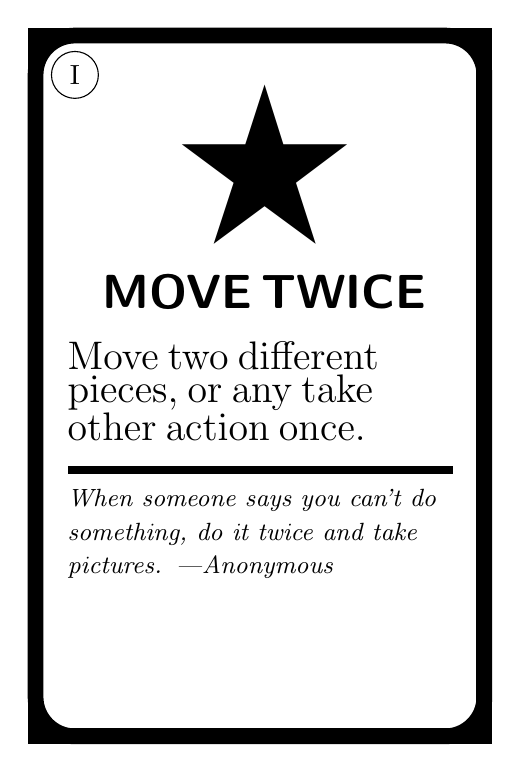
\begin{tikzpicture}
    \pgfmathsetmacro{\cardroundingradius}{5mm}
    \pgfmathsetmacro{\striproundingradius}{3mm}
    % \pgfmathsetmacro{\cardwidth}{5.9}
    % \pgfmathsetmacro{\cardheight}{9.2}
    \pgfmathsetmacro{\cardwidth}{5.7}
    \pgfmathsetmacro{\cardheight}{8.9}
    \pgfmathsetmacro{\stripwidth}{1.2}
    \pgfmathsetmacro{\strippadding}{0.1}
    \pgfmathsetmacro{\textpadding}{0.3}
    \pgfmathsetmacro{\ruleheight}{0.1}
    \providecommand{\stripfontsize}{\Huge}
    \providecommand{\captionfontsize}{\LARGE}
    \providecommand{\textfontsize}{\Large}
    \providecommand{\quotefontsize}{\small}
    \draw[line width=2mm,rounded corners=\cardroundingradius] (0,0) rectangle (\cardwidth,\cardheight);
    \draw[line width=2mm] (0,0) rectangle (\cardwidth,\cardheight);
    \node[text width=(\cardwidth-\strippadding-2*\textpadding)*1cm,below right,inner sep=0] at (\strippadding+\textpadding,\cardheight-\textpadding) 
    { 
    \begin{center} {\fontsize{80pt}{60pt}\selectfont \ding{72}}\\\end{center}
\begin{center}
    {\captionfontsize \textsf{\textbf{MOVE TWICE}}}\end{center}
        {\textfontsize Move two different pieces, or any take other action once.}\\
        \tikz{\fill (0,0) rectangle (\cardwidth-2*\strippadding-2*\textpadding,\ruleheight);}\\
        {\quotefontsize \textit{When someone says you can't do something, do it twice and take pictures. ---Anonymous}}\\[-2\baselineskip]
    };
    \node[circle,draw,text=black](c) at (.5,\cardheight-.5){I};
    \end{tikzpicture}%
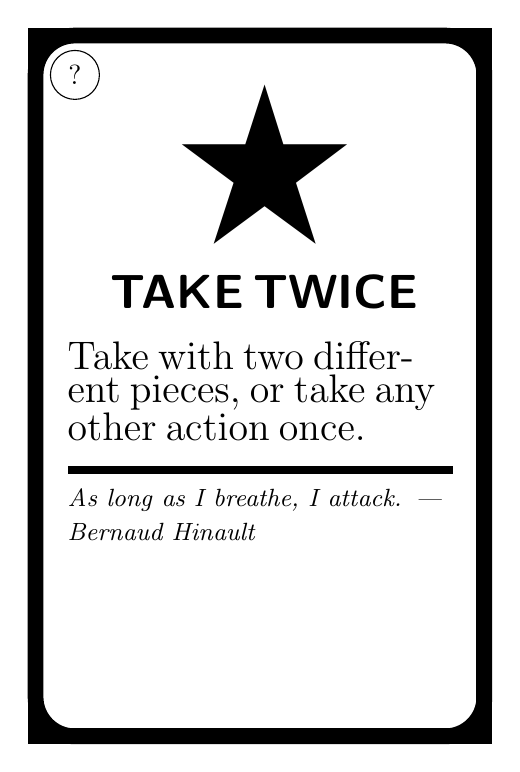
\begin{tikzpicture}
    \pgfmathsetmacro{\cardroundingradius}{5mm}
    \pgfmathsetmacro{\striproundingradius}{3mm}
    % \pgfmathsetmacro{\cardwidth}{5.9}
    % \pgfmathsetmacro{\cardheight}{9.2}
    \pgfmathsetmacro{\cardwidth}{5.7}
    \pgfmathsetmacro{\cardheight}{8.9}
    \pgfmathsetmacro{\stripwidth}{1.2}
    \pgfmathsetmacro{\strippadding}{0.1}
    \pgfmathsetmacro{\textpadding}{0.3}
    \pgfmathsetmacro{\ruleheight}{0.1}
    \providecommand{\stripfontsize}{\Huge}
    \providecommand{\captionfontsize}{\LARGE}
    \providecommand{\textfontsize}{\Large}
    \providecommand{\quotefontsize}{\small}
    \draw[line width=2mm,rounded corners=\cardroundingradius] (0,0) rectangle (\cardwidth,\cardheight);
    \draw[line width=2mm] (0,0) rectangle (\cardwidth,\cardheight);
    \node[text width=(\cardwidth-\strippadding-2*\textpadding)*1cm,below right,inner sep=0] at (\strippadding+\textpadding,\cardheight-\textpadding) 
    { 
    \begin{center} {\fontsize{80pt}{60pt}\selectfont \ding{72}}\\\end{center}
\begin{center}
    {\captionfontsize \textsf{\textbf{TAKE TWICE}}}\end{center}
        {\textfontsize Take with two different pieces, or take any other action once.}\\
        \tikz{\fill (0,0) rectangle (\cardwidth-2*\strippadding-2*\textpadding,\ruleheight);}\\
        {\quotefontsize \textit{As long as I breathe, I attack. ---Bernaud Hinault}}\\[-2\baselineskip]
    };
    \node[circle,draw,text=black](c) at (.5,\cardheight-.5){?};
    \end{tikzpicture}%
\begin{tikzpicture}
    \pgfmathsetmacro{\cardroundingradius}{5mm}
    \pgfmathsetmacro{\striproundingradius}{3mm}
    % \pgfmathsetmacro{\cardwidth}{5.9}
    % \pgfmathsetmacro{\cardheight}{9.2}
    \pgfmathsetmacro{\cardwidth}{5.7}
    \pgfmathsetmacro{\cardheight}{8.9}
    \pgfmathsetmacro{\stripwidth}{1.2}
    \pgfmathsetmacro{\strippadding}{0.1}
    \pgfmathsetmacro{\textpadding}{0.3}
    \pgfmathsetmacro{\ruleheight}{0.1}
    \providecommand{\stripfontsize}{\Huge}
    \providecommand{\captionfontsize}{\LARGE}
    \providecommand{\textfontsize}{\Large}
    \providecommand{\quotefontsize}{\small}
    \draw[line width=2mm,rounded corners=\cardroundingradius] (0,0) rectangle (\cardwidth,\cardheight);
    \draw[line width=2mm] (0,0) rectangle (\cardwidth,\cardheight);
    \node[text width=(\cardwidth-\strippadding-2*\textpadding)*1cm,below right,inner sep=0] at (\strippadding+\textpadding,\cardheight-\textpadding) 
    { 
    \begin{center} {\fontsize{80pt}{60pt}\selectfont ♘}\\\end{center}
\begin{center}
    {\captionfontsize \textsf{\textbf{LEND ME YOUR HORSE}}}\end{center}
        {\textfontsize Non-pawn pieces protected by a knight may also move/take like a knight.}\\
        \tikz{\fill (0,0) rectangle (\cardwidth-2*\strippadding-2*\textpadding,\ruleheight);}\\
        {\quotefontsize \textit{"You should know better than to mount another's war-horse", I said with a smirk. ---Jessica Leake}}\\[-2\baselineskip]
    };
    \node[circle,draw,text=black](c) at (.5,\cardheight-.5){C};
    \end{tikzpicture}%
\\[-\lineskip]
\begin{tikzpicture}
    \pgfmathsetmacro{\cardroundingradius}{5mm}
    \pgfmathsetmacro{\striproundingradius}{3mm}
    % \pgfmathsetmacro{\cardwidth}{5.9}
    % \pgfmathsetmacro{\cardheight}{9.2}
    \pgfmathsetmacro{\cardwidth}{5.7}
    \pgfmathsetmacro{\cardheight}{8.9}
    \pgfmathsetmacro{\stripwidth}{1.2}
    \pgfmathsetmacro{\strippadding}{0.1}
    \pgfmathsetmacro{\textpadding}{0.3}
    \pgfmathsetmacro{\ruleheight}{0.1}
    \providecommand{\stripfontsize}{\Huge}
    \providecommand{\captionfontsize}{\LARGE}
    \providecommand{\textfontsize}{\Large}
    \providecommand{\quotefontsize}{\small}
    \draw[line width=2mm,rounded corners=\cardroundingradius] (0,0) rectangle (\cardwidth,\cardheight);
    \draw[line width=2mm] (0,0) rectangle (\cardwidth,\cardheight);
    \node[text width=(\cardwidth-\strippadding-2*\textpadding)*1cm,below right,inner sep=0] at (\strippadding+\textpadding,\cardheight-\textpadding) 
    { 
    \begin{center} {\fontsize{80pt}{60pt}\selectfont ♘}\\\end{center}
\begin{center}
    {\captionfontsize \textsf{\textbf{JEDI KNIGHT}}}\end{center}
        {\textfontsize If you only have one knight on the board, it can also move and take like a Queen.}\\
        \tikz{\fill (0,0) rectangle (\cardwidth-2*\strippadding-2*\textpadding,\ruleheight);}\\
        {\quotefontsize \textit{If you strike me down, I shall become more powerful than you can possibly imagine. ---Obi-Wan Kenobi}}\\[-2\baselineskip]
    };
    \node[circle,draw,text=black](c) at (.5,\cardheight-.5){?};
    \end{tikzpicture}%
\begin{tikzpicture}
    \pgfmathsetmacro{\cardroundingradius}{5mm}
    \pgfmathsetmacro{\striproundingradius}{3mm}
    % \pgfmathsetmacro{\cardwidth}{5.9}
    % \pgfmathsetmacro{\cardheight}{9.2}
    \pgfmathsetmacro{\cardwidth}{5.7}
    \pgfmathsetmacro{\cardheight}{8.9}
    \pgfmathsetmacro{\stripwidth}{1.2}
    \pgfmathsetmacro{\strippadding}{0.1}
    \pgfmathsetmacro{\textpadding}{0.3}
    \pgfmathsetmacro{\ruleheight}{0.1}
    \providecommand{\stripfontsize}{\Huge}
    \providecommand{\captionfontsize}{\LARGE}
    \providecommand{\textfontsize}{\Large}
    \providecommand{\quotefontsize}{\small}
    \draw[line width=2mm,rounded corners=\cardroundingradius] (0,0) rectangle (\cardwidth,\cardheight);
    \draw[line width=2mm] (0,0) rectangle (\cardwidth,\cardheight);
    \node[text width=(\cardwidth-\strippadding-2*\textpadding)*1cm,below right,inner sep=0] at (\strippadding+\textpadding,\cardheight-\textpadding) 
    { 
    \begin{center} {\fontsize{80pt}{60pt}\selectfont ♙}\\\end{center}
\begin{center}
    {\captionfontsize \textsf{\textbf{BEROLINA PAWNS}}}\end{center}
        {\textfontsize Pawns move diagonally and take forward.}\\
        \tikz{\fill (0,0) rectangle (\cardwidth-2*\strippadding-2*\textpadding,\ruleheight);}\\
        {\quotefontsize \textit{Berolina is the female personification of Berlin and the allegorical female figure symbolizing the city. ---Wikipedia}}\\[-2\baselineskip]
    };
    \node[circle,draw,text=black](c) at (.5,\cardheight-.5){I};
    \end{tikzpicture}%
\begin{tikzpicture}
    \pgfmathsetmacro{\cardroundingradius}{5mm}
    \pgfmathsetmacro{\striproundingradius}{3mm}
    % \pgfmathsetmacro{\cardwidth}{5.9}
    % \pgfmathsetmacro{\cardheight}{9.2}
    \pgfmathsetmacro{\cardwidth}{5.7}
    \pgfmathsetmacro{\cardheight}{8.9}
    \pgfmathsetmacro{\stripwidth}{1.2}
    \pgfmathsetmacro{\strippadding}{0.1}
    \pgfmathsetmacro{\textpadding}{0.3}
    \pgfmathsetmacro{\ruleheight}{0.1}
    \providecommand{\stripfontsize}{\Huge}
    \providecommand{\captionfontsize}{\LARGE}
    \providecommand{\textfontsize}{\Large}
    \providecommand{\quotefontsize}{\small}
    \draw[line width=2mm,rounded corners=\cardroundingradius] (0,0) rectangle (\cardwidth,\cardheight);
    \draw[line width=2mm] (0,0) rectangle (\cardwidth,\cardheight);
    \node[text width=(\cardwidth-\strippadding-2*\textpadding)*1cm,below right,inner sep=0] at (\strippadding+\textpadding,\cardheight-\textpadding) 
    { 
    \begin{center} {\fontsize{80pt}{60pt}\selectfont ♙}\\\end{center}
\begin{center}
    {\captionfontsize \textsf{\textbf{BEROLINA PAWNS II}}}\end{center}
        {\textfontsize Pawns move diagonally. The take forward and sideways.}\\
        \tikz{\fill (0,0) rectangle (\cardwidth-2*\strippadding-2*\textpadding,\ruleheight);}\\
        {\quotefontsize \textit{Berolina is the female personification of Berlin and the allegorical female figure symbolizing the city. ---Wikipedia}}\\[-2\baselineskip]
    };
    \node[circle,draw,text=black](c) at (.5,\cardheight-.5){I};
    \end{tikzpicture}%
\begin{tikzpicture}
    \pgfmathsetmacro{\cardroundingradius}{5mm}
    \pgfmathsetmacro{\striproundingradius}{3mm}
    % \pgfmathsetmacro{\cardwidth}{5.9}
    % \pgfmathsetmacro{\cardheight}{9.2}
    \pgfmathsetmacro{\cardwidth}{5.7}
    \pgfmathsetmacro{\cardheight}{8.9}
    \pgfmathsetmacro{\stripwidth}{1.2}
    \pgfmathsetmacro{\strippadding}{0.1}
    \pgfmathsetmacro{\textpadding}{0.3}
    \pgfmathsetmacro{\ruleheight}{0.1}
    \providecommand{\stripfontsize}{\Huge}
    \providecommand{\captionfontsize}{\LARGE}
    \providecommand{\textfontsize}{\Large}
    \providecommand{\quotefontsize}{\small}
    \draw[line width=2mm,rounded corners=\cardroundingradius] (0,0) rectangle (\cardwidth,\cardheight);
    \draw[line width=2mm] (0,0) rectangle (\cardwidth,\cardheight);
    \node[text width=(\cardwidth-\strippadding-2*\textpadding)*1cm,below right,inner sep=0] at (\strippadding+\textpadding,\cardheight-\textpadding) 
    { 
    \begin{center} {\fontsize{80pt}{60pt}\selectfont ♙+}\\\end{center}
\begin{center}
    {\captionfontsize \textsf{\textbf{SHOGI PAWNS}}}\end{center}
        {\textfontsize Pawns move and take one square forward. Two Shogi Pawns may not be placed in the same file. Draw another card.}\\
        \tikz{\fill (0,0) rectangle (\cardwidth-2*\strippadding-2*\textpadding,\ruleheight);}\\
        {\quotefontsize \textit{If there is mate with a Pawn drop, there is a legal mate too. ---Shogi proverb}}\\[-2\baselineskip]
    };
    \node[circle,draw,text=black](c) at (.5,\cardheight-.5){S};
    \end{tikzpicture}%
\\[-\lineskip]
\begin{tikzpicture}
    \pgfmathsetmacro{\cardroundingradius}{5mm}
    \pgfmathsetmacro{\striproundingradius}{3mm}
    % \pgfmathsetmacro{\cardwidth}{5.9}
    % \pgfmathsetmacro{\cardheight}{9.2}
    \pgfmathsetmacro{\cardwidth}{5.7}
    \pgfmathsetmacro{\cardheight}{8.9}
    \pgfmathsetmacro{\stripwidth}{1.2}
    \pgfmathsetmacro{\strippadding}{0.1}
    \pgfmathsetmacro{\textpadding}{0.3}
    \pgfmathsetmacro{\ruleheight}{0.1}
    \providecommand{\stripfontsize}{\Huge}
    \providecommand{\captionfontsize}{\LARGE}
    \providecommand{\textfontsize}{\Large}
    \providecommand{\quotefontsize}{\small}
    \draw[line width=2mm,rounded corners=\cardroundingradius] (0,0) rectangle (\cardwidth,\cardheight);
    \draw[line width=2mm] (0,0) rectangle (\cardwidth,\cardheight);
    \node[text width=(\cardwidth-\strippadding-2*\textpadding)*1cm,below right,inner sep=0] at (\strippadding+\textpadding,\cardheight-\textpadding) 
    { 
    \begin{center} {\fontsize{80pt}{60pt}\selectfont ♙+}\\\end{center}
\begin{center}
    {\captionfontsize \textsf{\textbf{FAST PAWNS}}}\end{center}
        {\textfontsize Pawns capture normally, but may move any number of squares forward. Draw another card.}\\
        \tikz{\fill (0,0) rectangle (\cardwidth-2*\strippadding-2*\textpadding,\ruleheight);}\\
        {\quotefontsize \textit{ In ceremonies of the horsemen, even the pawn must hold a grudge. ---Bob Dylan}}\\[-2\baselineskip]
    };
    \node[circle,draw,text=black](c) at (.5,\cardheight-.5){?};
    \end{tikzpicture}%
\begin{tikzpicture}
    \pgfmathsetmacro{\cardroundingradius}{5mm}
    \pgfmathsetmacro{\striproundingradius}{3mm}
    % \pgfmathsetmacro{\cardwidth}{5.9}
    % \pgfmathsetmacro{\cardheight}{9.2}
    \pgfmathsetmacro{\cardwidth}{5.7}
    \pgfmathsetmacro{\cardheight}{8.9}
    \pgfmathsetmacro{\stripwidth}{1.2}
    \pgfmathsetmacro{\strippadding}{0.1}
    \pgfmathsetmacro{\textpadding}{0.3}
    \pgfmathsetmacro{\ruleheight}{0.1}
    \providecommand{\stripfontsize}{\Huge}
    \providecommand{\captionfontsize}{\LARGE}
    \providecommand{\textfontsize}{\Large}
    \providecommand{\quotefontsize}{\small}
    \draw[line width=2mm,rounded corners=\cardroundingradius] (0,0) rectangle (\cardwidth,\cardheight);
    \draw[line width=2mm] (0,0) rectangle (\cardwidth,\cardheight);
    \node[text width=(\cardwidth-\strippadding-2*\textpadding)*1cm,below right,inner sep=0] at (\strippadding+\textpadding,\cardheight-\textpadding) 
    { 
    \begin{center} {\fontsize{80pt}{60pt}\selectfont ♙+}\\\end{center}
\begin{center}
    {\captionfontsize \textsf{\textbf{BRIBE}}}\end{center}
        {\textfontsize On your turn you can do an action by an enemy pawn instead. Draw another card.}\\
        \tikz{\fill (0,0) rectangle (\cardwidth-2*\strippadding-2*\textpadding,\ruleheight);}\\
        {\quotefontsize \textit{Never underestimate the effectiveness of a straight cash bribe. ---Claud Cockburn}}\\[-2\baselineskip]
    };
    \node[circle,draw,text=black](c) at (.5,\cardheight-.5){?};
    \end{tikzpicture}%
\begin{tikzpicture}
    \pgfmathsetmacro{\cardroundingradius}{5mm}
    \pgfmathsetmacro{\striproundingradius}{3mm}
    % \pgfmathsetmacro{\cardwidth}{5.9}
    % \pgfmathsetmacro{\cardheight}{9.2}
    \pgfmathsetmacro{\cardwidth}{5.7}
    \pgfmathsetmacro{\cardheight}{8.9}
    \pgfmathsetmacro{\stripwidth}{1.2}
    \pgfmathsetmacro{\strippadding}{0.1}
    \pgfmathsetmacro{\textpadding}{0.3}
    \pgfmathsetmacro{\ruleheight}{0.1}
    \providecommand{\stripfontsize}{\Huge}
    \providecommand{\captionfontsize}{\LARGE}
    \providecommand{\textfontsize}{\Large}
    \providecommand{\quotefontsize}{\small}
    \draw[line width=2mm,rounded corners=\cardroundingradius] (0,0) rectangle (\cardwidth,\cardheight);
    \draw[line width=2mm] (0,0) rectangle (\cardwidth,\cardheight);
    \node[text width=(\cardwidth-\strippadding-2*\textpadding)*1cm,below right,inner sep=0] at (\strippadding+\textpadding,\cardheight-\textpadding) 
    { 
    \begin{center} {\fontsize{80pt}{60pt}\selectfont ♙}\\\end{center}
\begin{center}
    {\captionfontsize \textsf{\textbf{CHINESE CHECKERS}}}\end{center}
        {\textfontsize Pawns take normally, but move like Chinese checkers.}\\
        \tikz{\fill (0,0) rectangle (\cardwidth-2*\strippadding-2*\textpadding,\ruleheight);}\\
        {\quotefontsize \textit{\tiny The Pentagon banned the army from using Chinese-made berets. In a more veiled slap at the Chinese, the Pentagon also banned any alternative form of checkers. ---Jimmy Fallon}}\\[-2\baselineskip]
    };
    \node[circle,draw,text=black](c) at (.5,\cardheight-.5){?};
    \end{tikzpicture}%
\begin{tikzpicture}
    \pgfmathsetmacro{\cardroundingradius}{5mm}
    \pgfmathsetmacro{\striproundingradius}{3mm}
    % \pgfmathsetmacro{\cardwidth}{5.9}
    % \pgfmathsetmacro{\cardheight}{9.2}
    \pgfmathsetmacro{\cardwidth}{5.7}
    \pgfmathsetmacro{\cardheight}{8.9}
    \pgfmathsetmacro{\stripwidth}{1.2}
    \pgfmathsetmacro{\strippadding}{0.1}
    \pgfmathsetmacro{\textpadding}{0.3}
    \pgfmathsetmacro{\ruleheight}{0.1}
    \providecommand{\stripfontsize}{\Huge}
    \providecommand{\captionfontsize}{\LARGE}
    \providecommand{\textfontsize}{\Large}
    \providecommand{\quotefontsize}{\small}
    \draw[line width=2mm,rounded corners=\cardroundingradius] (0,0) rectangle (\cardwidth,\cardheight);
    \draw[line width=2mm] (0,0) rectangle (\cardwidth,\cardheight);
    \node[text width=(\cardwidth-\strippadding-2*\textpadding)*1cm,below right,inner sep=0] at (\strippadding+\textpadding,\cardheight-\textpadding) 
    { 
    \begin{center} {\fontsize{80pt}{60pt}\selectfont ♘}\\\end{center}
\begin{center}
    {\captionfontsize \textsf{\textbf{NIGHT WIZARD}}}\end{center}
        {\textfontsize Move/take life a giraffe [1,3], or one square diagonally [1,1].}\\
        \tikz{\fill (0,0) rectangle (\cardwidth-2*\strippadding-2*\textpadding,\ruleheight);}\\
        {\quotefontsize \textit{Do not meddle in the affairs of Wizards, for they are subtle and quick to anger. ---J. R. R. Tolkien}}\\[-2\baselineskip]
    };
    \node[circle,draw,text=black](c) at (.5,\cardheight-.5){Ω};
    \end{tikzpicture}%
\\[-\lineskip]
\begin{tikzpicture}
    \pgfmathsetmacro{\cardroundingradius}{5mm}
    \pgfmathsetmacro{\striproundingradius}{3mm}
    % \pgfmathsetmacro{\cardwidth}{5.9}
    % \pgfmathsetmacro{\cardheight}{9.2}
    \pgfmathsetmacro{\cardwidth}{5.7}
    \pgfmathsetmacro{\cardheight}{8.9}
    \pgfmathsetmacro{\stripwidth}{1.2}
    \pgfmathsetmacro{\strippadding}{0.1}
    \pgfmathsetmacro{\textpadding}{0.3}
    \pgfmathsetmacro{\ruleheight}{0.1}
    \providecommand{\stripfontsize}{\Huge}
    \providecommand{\captionfontsize}{\LARGE}
    \providecommand{\textfontsize}{\Large}
    \providecommand{\quotefontsize}{\small}
    \draw[line width=2mm,rounded corners=\cardroundingradius] (0,0) rectangle (\cardwidth,\cardheight);
    \draw[line width=2mm] (0,0) rectangle (\cardwidth,\cardheight);
    \node[text width=(\cardwidth-\strippadding-2*\textpadding)*1cm,below right,inner sep=0] at (\strippadding+\textpadding,\cardheight-\textpadding) 
    { 
    \begin{center} {\fontsize{80pt}{60pt}\selectfont ♘}\\\end{center}
\begin{center}
    {\captionfontsize \textsf{\textbf{TALLADEGA KNIGHTS}}}\end{center}
        {\textfontsize Knights on your color may move/take like Rooks. Knights on your opponents colore may move/take like Bishops.}\\
        \tikz{\fill (0,0) rectangle (\cardwidth-2*\strippadding-2*\textpadding,\ruleheight);}\\
        {\quotefontsize \textit{If you ain't first, you're last. ---Ricky Bobby}}\\[-2\baselineskip]
    };
    \node[circle,draw,text=black](c) at (.5,\cardheight-.5){C};
    \end{tikzpicture}%
\begin{tikzpicture}
    \pgfmathsetmacro{\cardroundingradius}{5mm}
    \pgfmathsetmacro{\striproundingradius}{3mm}
    % \pgfmathsetmacro{\cardwidth}{5.9}
    % \pgfmathsetmacro{\cardheight}{9.2}
    \pgfmathsetmacro{\cardwidth}{5.7}
    \pgfmathsetmacro{\cardheight}{8.9}
    \pgfmathsetmacro{\stripwidth}{1.2}
    \pgfmathsetmacro{\strippadding}{0.1}
    \pgfmathsetmacro{\textpadding}{0.3}
    \pgfmathsetmacro{\ruleheight}{0.1}
    \providecommand{\stripfontsize}{\Huge}
    \providecommand{\captionfontsize}{\LARGE}
    \providecommand{\textfontsize}{\Large}
    \providecommand{\quotefontsize}{\small}
    \draw[line width=2mm,rounded corners=\cardroundingradius] (0,0) rectangle (\cardwidth,\cardheight);
    \draw[line width=2mm] (0,0) rectangle (\cardwidth,\cardheight);
    \node[text width=(\cardwidth-\strippadding-2*\textpadding)*1cm,below right,inner sep=0] at (\strippadding+\textpadding,\cardheight-\textpadding) 
    { 
    \begin{center} {\fontsize{80pt}{60pt}\selectfont ♔+}\\\end{center}
\begin{center}
    {\captionfontsize \textsf{\textbf{TOUCHDOWN}}}\end{center}
        {\textfontsize If your king is on the last rank at the end of your turn, you win.}\\
        \tikz{\fill (0,0) rectangle (\cardwidth-2*\strippadding-2*\textpadding,\ruleheight);}\\
        {\quotefontsize \textit{It's one of those things: I would 100 percent pancake a guy and steal his soul over scoring a touchdown. ---George Kittle}}\\[-2\baselineskip]
    };
    \node[circle,draw,text=black](c) at (.5,\cardheight-.5){?};
    \end{tikzpicture}%
\begin{tikzpicture}
    \pgfmathsetmacro{\cardroundingradius}{5mm}
    \pgfmathsetmacro{\striproundingradius}{3mm}
    % \pgfmathsetmacro{\cardwidth}{5.9}
    % \pgfmathsetmacro{\cardheight}{9.2}
    \pgfmathsetmacro{\cardwidth}{5.7}
    \pgfmathsetmacro{\cardheight}{8.9}
    \pgfmathsetmacro{\stripwidth}{1.2}
    \pgfmathsetmacro{\strippadding}{0.1}
    \pgfmathsetmacro{\textpadding}{0.3}
    \pgfmathsetmacro{\ruleheight}{0.1}
    \providecommand{\stripfontsize}{\Huge}
    \providecommand{\captionfontsize}{\LARGE}
    \providecommand{\textfontsize}{\Large}
    \providecommand{\quotefontsize}{\small}
    \draw[line width=2mm,rounded corners=\cardroundingradius] (0,0) rectangle (\cardwidth,\cardheight);
    \draw[line width=2mm] (0,0) rectangle (\cardwidth,\cardheight);
    \node[text width=(\cardwidth-\strippadding-2*\textpadding)*1cm,below right,inner sep=0] at (\strippadding+\textpadding,\cardheight-\textpadding) 
    { 
    \begin{center} {\fontsize{80pt}{60pt}\selectfont ♔+}\\\end{center}
\begin{center}
    {\captionfontsize \textsf{\textbf{SUMO KING}}}\end{center}
        {\textfontsize Kings may take normally or shove billiards style. Pieces that fall of the edge die.}\\
        \tikz{\fill (0,0) rectangle (\cardwidth-2*\strippadding-2*\textpadding,\ruleheight);}\\
        {\quotefontsize \textit{Good spirit! But you should push an opponent with more force! ---E. Honda}}\\[-2\baselineskip]
    };
    \node[circle,draw,text=black](c) at (.5,\cardheight-.5){C};
    \end{tikzpicture}%
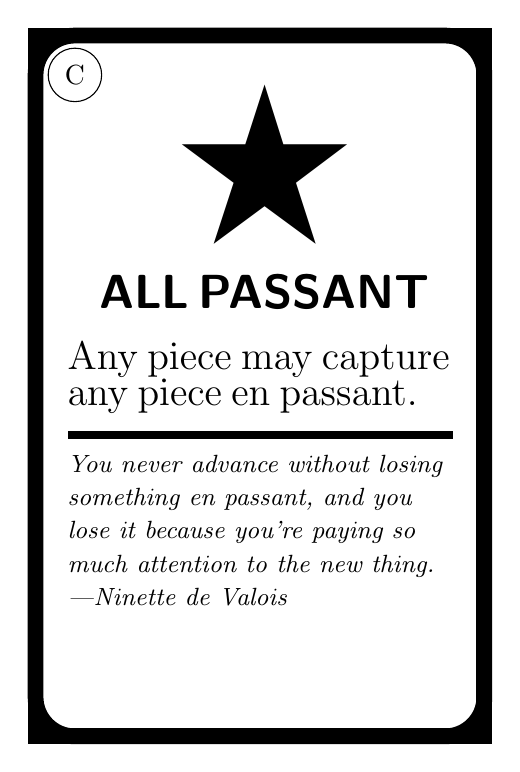
\begin{tikzpicture}
    \pgfmathsetmacro{\cardroundingradius}{5mm}
    \pgfmathsetmacro{\striproundingradius}{3mm}
    % \pgfmathsetmacro{\cardwidth}{5.9}
    % \pgfmathsetmacro{\cardheight}{9.2}
    \pgfmathsetmacro{\cardwidth}{5.7}
    \pgfmathsetmacro{\cardheight}{8.9}
    \pgfmathsetmacro{\stripwidth}{1.2}
    \pgfmathsetmacro{\strippadding}{0.1}
    \pgfmathsetmacro{\textpadding}{0.3}
    \pgfmathsetmacro{\ruleheight}{0.1}
    \providecommand{\stripfontsize}{\Huge}
    \providecommand{\captionfontsize}{\LARGE}
    \providecommand{\textfontsize}{\Large}
    \providecommand{\quotefontsize}{\small}
    \draw[line width=2mm,rounded corners=\cardroundingradius] (0,0) rectangle (\cardwidth,\cardheight);
    \draw[line width=2mm] (0,0) rectangle (\cardwidth,\cardheight);
    \node[text width=(\cardwidth-\strippadding-2*\textpadding)*1cm,below right,inner sep=0] at (\strippadding+\textpadding,\cardheight-\textpadding) 
    { 
    \begin{center} {\fontsize{80pt}{60pt}\selectfont \ding{72}}\\\end{center}
\begin{center}
    {\captionfontsize \textsf{\textbf{ALL PASSANT}}}\end{center}
        {\textfontsize Any piece may capture any piece en passant.}\\
        \tikz{\fill (0,0) rectangle (\cardwidth-2*\strippadding-2*\textpadding,\ruleheight);}\\
        {\quotefontsize \textit{You never advance without losing something en passant, and you lose it because you're paying so much attention to the new thing. ---Ninette de Valois}}\\[-2\baselineskip]
    };
    \node[circle,draw,text=black](c) at (.5,\cardheight-.5){C};
    \end{tikzpicture}%
\\[-\lineskip]
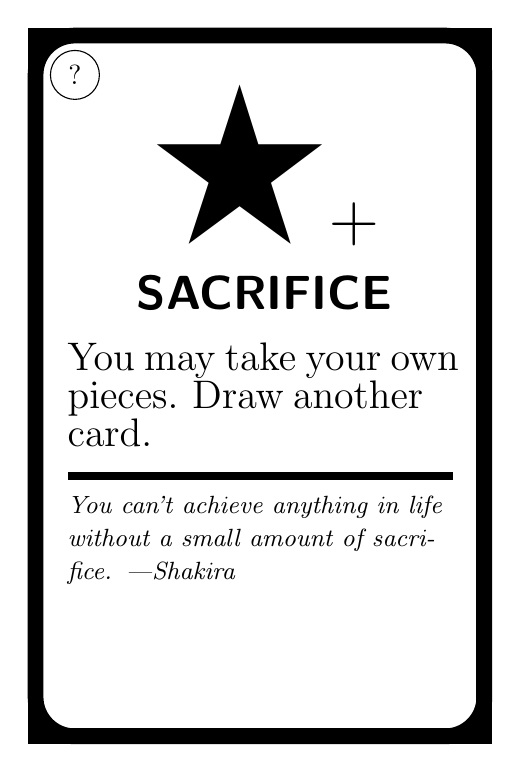
\begin{tikzpicture}
    \pgfmathsetmacro{\cardroundingradius}{5mm}
    \pgfmathsetmacro{\striproundingradius}{3mm}
    % \pgfmathsetmacro{\cardwidth}{5.9}
    % \pgfmathsetmacro{\cardheight}{9.2}
    \pgfmathsetmacro{\cardwidth}{5.7}
    \pgfmathsetmacro{\cardheight}{8.9}
    \pgfmathsetmacro{\stripwidth}{1.2}
    \pgfmathsetmacro{\strippadding}{0.1}
    \pgfmathsetmacro{\textpadding}{0.3}
    \pgfmathsetmacro{\ruleheight}{0.1}
    \providecommand{\stripfontsize}{\Huge}
    \providecommand{\captionfontsize}{\LARGE}
    \providecommand{\textfontsize}{\Large}
    \providecommand{\quotefontsize}{\small}
    \draw[line width=2mm,rounded corners=\cardroundingradius] (0,0) rectangle (\cardwidth,\cardheight);
    \draw[line width=2mm] (0,0) rectangle (\cardwidth,\cardheight);
    \node[text width=(\cardwidth-\strippadding-2*\textpadding)*1cm,below right,inner sep=0] at (\strippadding+\textpadding,\cardheight-\textpadding) 
    { 
    \begin{center} {\fontsize{80pt}{60pt}\selectfont \ding{72}+}\\\end{center}
\begin{center}
    {\captionfontsize \textsf{\textbf{SACRIFICE}}}\end{center}
        {\textfontsize You may take your own pieces. Draw another card.}\\
        \tikz{\fill (0,0) rectangle (\cardwidth-2*\strippadding-2*\textpadding,\ruleheight);}\\
        {\quotefontsize \textit{You can't achieve anything in life without a small amount of sacrifice. ---Shakira}}\\[-2\baselineskip]
    };
    \node[circle,draw,text=black](c) at (.5,\cardheight-.5){?};
    \end{tikzpicture}%
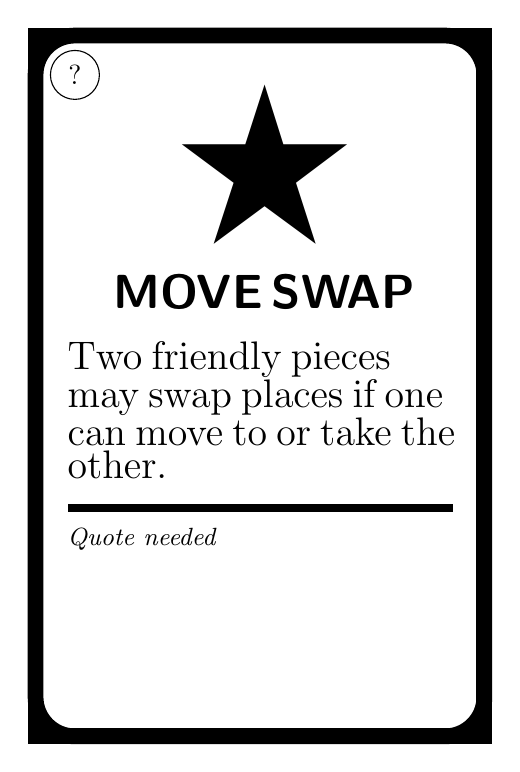
\begin{tikzpicture}
    \pgfmathsetmacro{\cardroundingradius}{5mm}
    \pgfmathsetmacro{\striproundingradius}{3mm}
    % \pgfmathsetmacro{\cardwidth}{5.9}
    % \pgfmathsetmacro{\cardheight}{9.2}
    \pgfmathsetmacro{\cardwidth}{5.7}
    \pgfmathsetmacro{\cardheight}{8.9}
    \pgfmathsetmacro{\stripwidth}{1.2}
    \pgfmathsetmacro{\strippadding}{0.1}
    \pgfmathsetmacro{\textpadding}{0.3}
    \pgfmathsetmacro{\ruleheight}{0.1}
    \providecommand{\stripfontsize}{\Huge}
    \providecommand{\captionfontsize}{\LARGE}
    \providecommand{\textfontsize}{\Large}
    \providecommand{\quotefontsize}{\small}
    \draw[line width=2mm,rounded corners=\cardroundingradius] (0,0) rectangle (\cardwidth,\cardheight);
    \draw[line width=2mm] (0,0) rectangle (\cardwidth,\cardheight);
    \node[text width=(\cardwidth-\strippadding-2*\textpadding)*1cm,below right,inner sep=0] at (\strippadding+\textpadding,\cardheight-\textpadding) 
    { 
    \begin{center} {\fontsize{80pt}{60pt}\selectfont \ding{72}}\\\end{center}
\begin{center}
    {\captionfontsize \textsf{\textbf{MOVE SWAP}}}\end{center}
        {\textfontsize Two friendly pieces may swap places if one can move to or take the other.}\\
        \tikz{\fill (0,0) rectangle (\cardwidth-2*\strippadding-2*\textpadding,\ruleheight);}\\
        {\quotefontsize \textit{Quote needed}}\\[-2\baselineskip]
    };
    \node[circle,draw,text=black](c) at (.5,\cardheight-.5){?};
    \end{tikzpicture}%
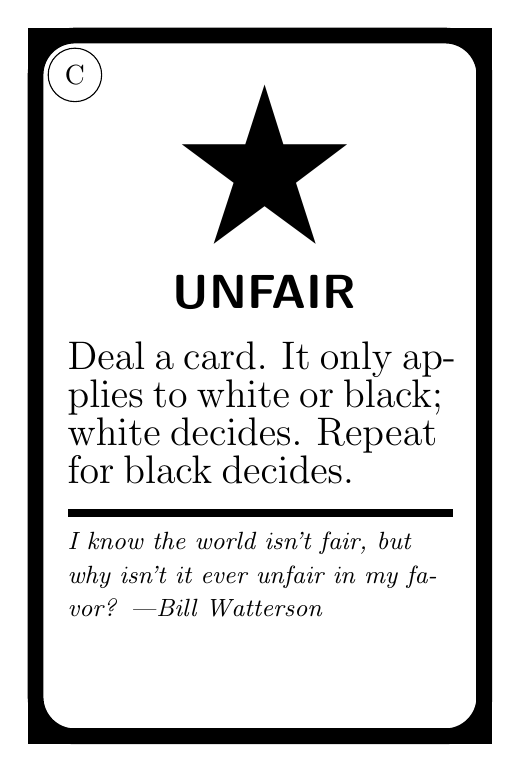
\begin{tikzpicture}
    \pgfmathsetmacro{\cardroundingradius}{5mm}
    \pgfmathsetmacro{\striproundingradius}{3mm}
    % \pgfmathsetmacro{\cardwidth}{5.9}
    % \pgfmathsetmacro{\cardheight}{9.2}
    \pgfmathsetmacro{\cardwidth}{5.7}
    \pgfmathsetmacro{\cardheight}{8.9}
    \pgfmathsetmacro{\stripwidth}{1.2}
    \pgfmathsetmacro{\strippadding}{0.1}
    \pgfmathsetmacro{\textpadding}{0.3}
    \pgfmathsetmacro{\ruleheight}{0.1}
    \providecommand{\stripfontsize}{\Huge}
    \providecommand{\captionfontsize}{\LARGE}
    \providecommand{\textfontsize}{\Large}
    \providecommand{\quotefontsize}{\small}
    \draw[line width=2mm,rounded corners=\cardroundingradius] (0,0) rectangle (\cardwidth,\cardheight);
    \draw[line width=2mm] (0,0) rectangle (\cardwidth,\cardheight);
    \node[text width=(\cardwidth-\strippadding-2*\textpadding)*1cm,below right,inner sep=0] at (\strippadding+\textpadding,\cardheight-\textpadding) 
    { 
    \begin{center} {\fontsize{80pt}{60pt}\selectfont \ding{72}}\\\end{center}
\begin{center}
    {\captionfontsize \textsf{\textbf{UNFAIR}}}\end{center}
        {\textfontsize Deal a card. It only applies to white or black; white decides. Repeat for black decides.}\\
        \tikz{\fill (0,0) rectangle (\cardwidth-2*\strippadding-2*\textpadding,\ruleheight);}\\
        {\quotefontsize \textit{I know the world isn't fair, but why isn't it ever unfair in my favor? ---Bill Watterson}}\\[-2\baselineskip]
    };
    \node[circle,draw,text=black](c) at (.5,\cardheight-.5){C};
    \end{tikzpicture}%
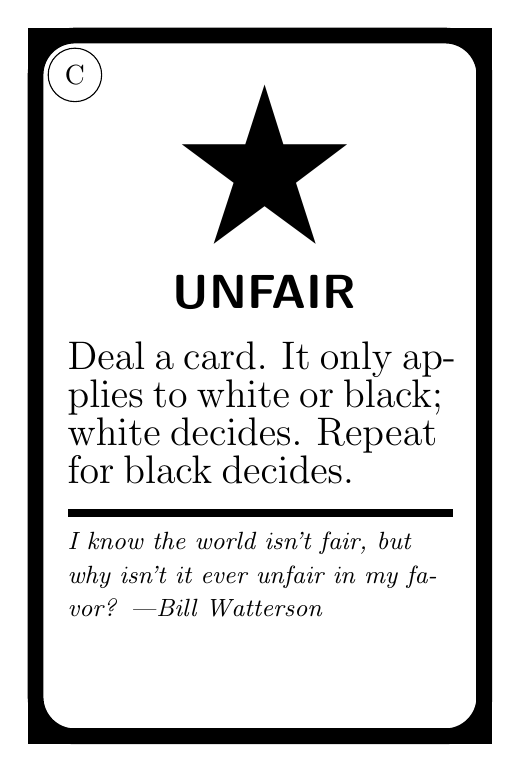
\begin{tikzpicture}
    \pgfmathsetmacro{\cardroundingradius}{5mm}
    \pgfmathsetmacro{\striproundingradius}{3mm}
    % \pgfmathsetmacro{\cardwidth}{5.9}
    % \pgfmathsetmacro{\cardheight}{9.2}
    \pgfmathsetmacro{\cardwidth}{5.7}
    \pgfmathsetmacro{\cardheight}{8.9}
    \pgfmathsetmacro{\stripwidth}{1.2}
    \pgfmathsetmacro{\strippadding}{0.1}
    \pgfmathsetmacro{\textpadding}{0.3}
    \pgfmathsetmacro{\ruleheight}{0.1}
    \providecommand{\stripfontsize}{\Huge}
    \providecommand{\captionfontsize}{\LARGE}
    \providecommand{\textfontsize}{\Large}
    \providecommand{\quotefontsize}{\small}
    \draw[line width=2mm,rounded corners=\cardroundingradius] (0,0) rectangle (\cardwidth,\cardheight);
    \draw[line width=2mm] (0,0) rectangle (\cardwidth,\cardheight);
    \node[text width=(\cardwidth-\strippadding-2*\textpadding)*1cm,below right,inner sep=0] at (\strippadding+\textpadding,\cardheight-\textpadding) 
    { 
    \begin{center} {\fontsize{80pt}{60pt}\selectfont \ding{72}}\\\end{center}
\begin{center}
    {\captionfontsize \textsf{\textbf{UNFAIR}}}\end{center}
        {\textfontsize Deal a card. It only applies to white or black; white decides. Repeat for black decides.}\\
        \tikz{\fill (0,0) rectangle (\cardwidth-2*\strippadding-2*\textpadding,\ruleheight);}\\
        {\quotefontsize \textit{I know the world isn't fair, but why isn't it ever unfair in my favor? ---Bill Watterson}}\\[-2\baselineskip]
    };
    \node[circle,draw,text=black](c) at (.5,\cardheight-.5){C};
    \end{tikzpicture}%
\\[-\lineskip]
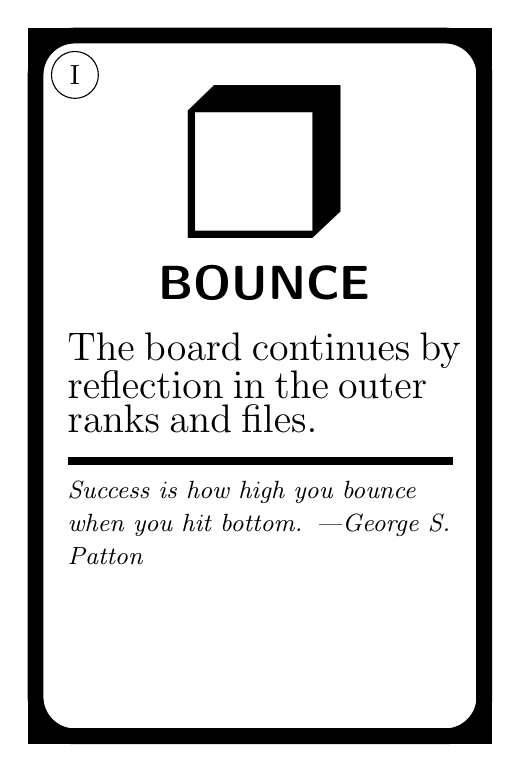
\begin{tikzpicture}
    \pgfmathsetmacro{\cardroundingradius}{5mm}
    \pgfmathsetmacro{\striproundingradius}{3mm}
    % \pgfmathsetmacro{\cardwidth}{5.9}
    % \pgfmathsetmacro{\cardheight}{9.2}
    \pgfmathsetmacro{\cardwidth}{5.7}
    \pgfmathsetmacro{\cardheight}{8.9}
    \pgfmathsetmacro{\stripwidth}{1.2}
    \pgfmathsetmacro{\strippadding}{0.1}
    \pgfmathsetmacro{\textpadding}{0.3}
    \pgfmathsetmacro{\ruleheight}{0.1}
    \providecommand{\stripfontsize}{\Huge}
    \providecommand{\captionfontsize}{\LARGE}
    \providecommand{\textfontsize}{\Large}
    \providecommand{\quotefontsize}{\small}
    \draw[line width=2mm,rounded corners=\cardroundingradius] (0,0) rectangle (\cardwidth,\cardheight);
    \draw[line width=2mm] (0,0) rectangle (\cardwidth,\cardheight);
    \node[text width=(\cardwidth-\strippadding-2*\textpadding)*1cm,below right,inner sep=0] at (\strippadding+\textpadding,\cardheight-\textpadding) 
    { 
    \begin{center} {\fontsize{80pt}{60pt}\selectfont \ding{114}}\\\end{center}
\begin{center}
    {\captionfontsize \textsf{\textbf{BOUNCE}}}\end{center}
        {\textfontsize The board continues by reflection in the outer ranks and files.}\\
        \tikz{\fill (0,0) rectangle (\cardwidth-2*\strippadding-2*\textpadding,\ruleheight);}\\
        {\quotefontsize \textit{Success is how high you bounce when you hit bottom. ---George S. Patton}}\\[-2\baselineskip]
    };
    \node[circle,draw,text=black](c) at (.5,\cardheight-.5){I};
    \end{tikzpicture}%
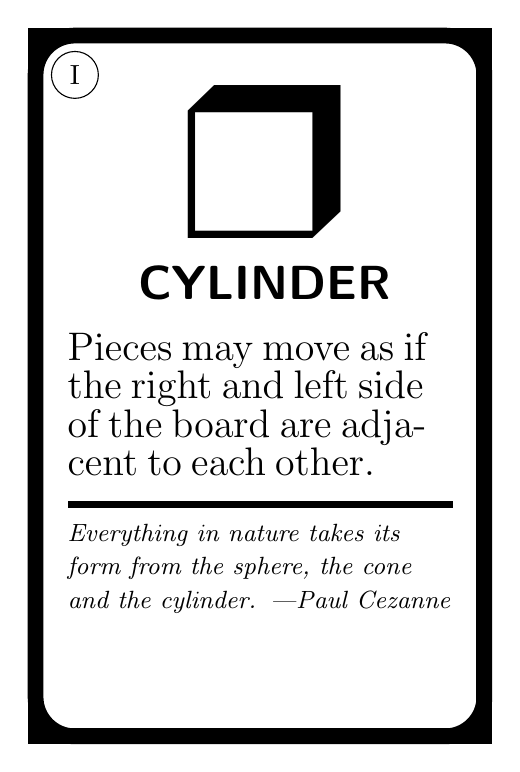
\begin{tikzpicture}
    \pgfmathsetmacro{\cardroundingradius}{5mm}
    \pgfmathsetmacro{\striproundingradius}{3mm}
    % \pgfmathsetmacro{\cardwidth}{5.9}
    % \pgfmathsetmacro{\cardheight}{9.2}
    \pgfmathsetmacro{\cardwidth}{5.7}
    \pgfmathsetmacro{\cardheight}{8.9}
    \pgfmathsetmacro{\stripwidth}{1.2}
    \pgfmathsetmacro{\strippadding}{0.1}
    \pgfmathsetmacro{\textpadding}{0.3}
    \pgfmathsetmacro{\ruleheight}{0.1}
    \providecommand{\stripfontsize}{\Huge}
    \providecommand{\captionfontsize}{\LARGE}
    \providecommand{\textfontsize}{\Large}
    \providecommand{\quotefontsize}{\small}
    \draw[line width=2mm,rounded corners=\cardroundingradius] (0,0) rectangle (\cardwidth,\cardheight);
    \draw[line width=2mm] (0,0) rectangle (\cardwidth,\cardheight);
    \node[text width=(\cardwidth-\strippadding-2*\textpadding)*1cm,below right,inner sep=0] at (\strippadding+\textpadding,\cardheight-\textpadding) 
    { 
    \begin{center} {\fontsize{80pt}{60pt}\selectfont \ding{114}}\\\end{center}
\begin{center}
    {\captionfontsize \textsf{\textbf{CYLINDER}}}\end{center}
        {\textfontsize Pieces may move as if the right and left side of the board are adjacent to each other.}\\
        \tikz{\fill (0,0) rectangle (\cardwidth-2*\strippadding-2*\textpadding,\ruleheight);}\\
        {\quotefontsize \textit{Everything in nature takes its form from the sphere, the cone and the cylinder. ---Paul Cezanne}}\\[-2\baselineskip]
    };
    \node[circle,draw,text=black](c) at (.5,\cardheight-.5){I};
    \end{tikzpicture}%
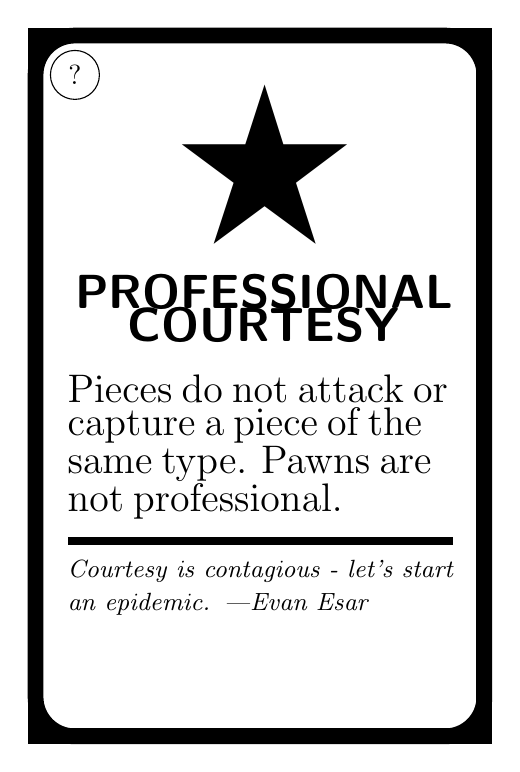
\begin{tikzpicture}
    \pgfmathsetmacro{\cardroundingradius}{5mm}
    \pgfmathsetmacro{\striproundingradius}{3mm}
    % \pgfmathsetmacro{\cardwidth}{5.9}
    % \pgfmathsetmacro{\cardheight}{9.2}
    \pgfmathsetmacro{\cardwidth}{5.7}
    \pgfmathsetmacro{\cardheight}{8.9}
    \pgfmathsetmacro{\stripwidth}{1.2}
    \pgfmathsetmacro{\strippadding}{0.1}
    \pgfmathsetmacro{\textpadding}{0.3}
    \pgfmathsetmacro{\ruleheight}{0.1}
    \providecommand{\stripfontsize}{\Huge}
    \providecommand{\captionfontsize}{\LARGE}
    \providecommand{\textfontsize}{\Large}
    \providecommand{\quotefontsize}{\small}
    \draw[line width=2mm,rounded corners=\cardroundingradius] (0,0) rectangle (\cardwidth,\cardheight);
    \draw[line width=2mm] (0,0) rectangle (\cardwidth,\cardheight);
    \node[text width=(\cardwidth-\strippadding-2*\textpadding)*1cm,below right,inner sep=0] at (\strippadding+\textpadding,\cardheight-\textpadding) 
    { 
    \begin{center} {\fontsize{80pt}{60pt}\selectfont \ding{72}}\\\end{center}
\begin{center}
    {\captionfontsize \textsf{\textbf{PROFESSIONAL COURTESY}}}\end{center}
        {\textfontsize Pieces do not attack or capture a piece of the same type. Pawns are not professional.}\\
        \tikz{\fill (0,0) rectangle (\cardwidth-2*\strippadding-2*\textpadding,\ruleheight);}\\
        {\quotefontsize \textit{Courtesy is contagious - let's start an epidemic. ---Evan Esar}}\\[-2\baselineskip]
    };
    \node[circle,draw,text=black](c) at (.5,\cardheight-.5){?};
    \end{tikzpicture}%
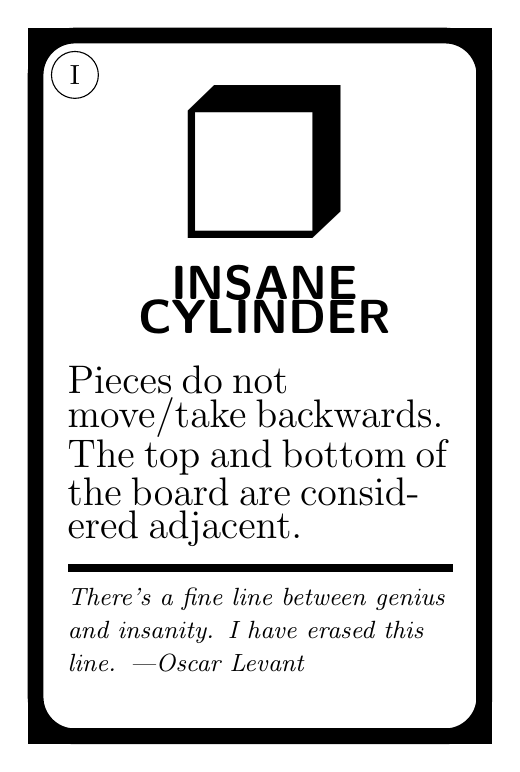
\begin{tikzpicture}
    \pgfmathsetmacro{\cardroundingradius}{5mm}
    \pgfmathsetmacro{\striproundingradius}{3mm}
    % \pgfmathsetmacro{\cardwidth}{5.9}
    % \pgfmathsetmacro{\cardheight}{9.2}
    \pgfmathsetmacro{\cardwidth}{5.7}
    \pgfmathsetmacro{\cardheight}{8.9}
    \pgfmathsetmacro{\stripwidth}{1.2}
    \pgfmathsetmacro{\strippadding}{0.1}
    \pgfmathsetmacro{\textpadding}{0.3}
    \pgfmathsetmacro{\ruleheight}{0.1}
    \providecommand{\stripfontsize}{\Huge}
    \providecommand{\captionfontsize}{\LARGE}
    \providecommand{\textfontsize}{\Large}
    \providecommand{\quotefontsize}{\small}
    \draw[line width=2mm,rounded corners=\cardroundingradius] (0,0) rectangle (\cardwidth,\cardheight);
    \draw[line width=2mm] (0,0) rectangle (\cardwidth,\cardheight);
    \node[text width=(\cardwidth-\strippadding-2*\textpadding)*1cm,below right,inner sep=0] at (\strippadding+\textpadding,\cardheight-\textpadding) 
    { 
    \begin{center} {\fontsize{80pt}{60pt}\selectfont \ding{114}}\\\end{center}
\begin{center}
    {\captionfontsize \textsf{\textbf{INSANE CYLINDER}}}\end{center}
        {\textfontsize Pieces do not move/take backwards. The top and bottom of the board are considered adjacent.}\\
        \tikz{\fill (0,0) rectangle (\cardwidth-2*\strippadding-2*\textpadding,\ruleheight);}\\
        {\quotefontsize \textit{There's a fine line between genius and insanity. I have erased this line. ---Oscar Levant}}\\[-2\baselineskip]
    };
    \node[circle,draw,text=black](c) at (.5,\cardheight-.5){I};
    \end{tikzpicture}%
\\[-\lineskip]
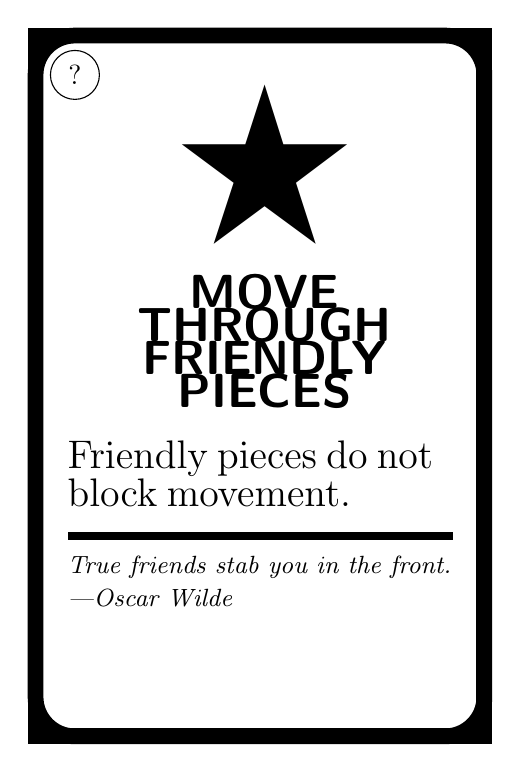
\begin{tikzpicture}
    \pgfmathsetmacro{\cardroundingradius}{5mm}
    \pgfmathsetmacro{\striproundingradius}{3mm}
    % \pgfmathsetmacro{\cardwidth}{5.9}
    % \pgfmathsetmacro{\cardheight}{9.2}
    \pgfmathsetmacro{\cardwidth}{5.7}
    \pgfmathsetmacro{\cardheight}{8.9}
    \pgfmathsetmacro{\stripwidth}{1.2}
    \pgfmathsetmacro{\strippadding}{0.1}
    \pgfmathsetmacro{\textpadding}{0.3}
    \pgfmathsetmacro{\ruleheight}{0.1}
    \providecommand{\stripfontsize}{\Huge}
    \providecommand{\captionfontsize}{\LARGE}
    \providecommand{\textfontsize}{\Large}
    \providecommand{\quotefontsize}{\small}
    \draw[line width=2mm,rounded corners=\cardroundingradius] (0,0) rectangle (\cardwidth,\cardheight);
    \draw[line width=2mm] (0,0) rectangle (\cardwidth,\cardheight);
    \node[text width=(\cardwidth-\strippadding-2*\textpadding)*1cm,below right,inner sep=0] at (\strippadding+\textpadding,\cardheight-\textpadding) 
    { 
    \begin{center} {\fontsize{80pt}{60pt}\selectfont \ding{72}}\\\end{center}
\begin{center}
    {\captionfontsize \textsf{\textbf{MOVE THROUGH FRIENDLY PIECES}}}\end{center}
        {\textfontsize Friendly pieces do not block movement.}\\
        \tikz{\fill (0,0) rectangle (\cardwidth-2*\strippadding-2*\textpadding,\ruleheight);}\\
        {\quotefontsize \textit{True friends stab you in the front. ---Oscar Wilde}}\\[-2\baselineskip]
    };
    \node[circle,draw,text=black](c) at (.5,\cardheight-.5){?};
    \end{tikzpicture}%
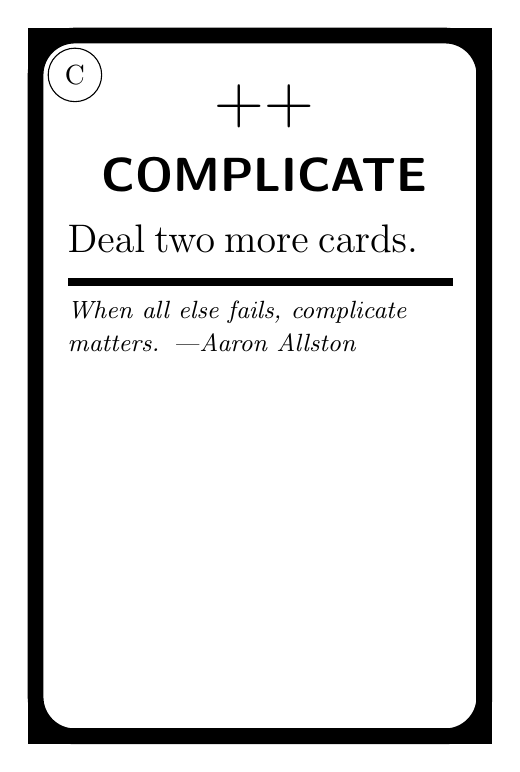
\begin{tikzpicture}
    \pgfmathsetmacro{\cardroundingradius}{5mm}
    \pgfmathsetmacro{\striproundingradius}{3mm}
    % \pgfmathsetmacro{\cardwidth}{5.9}
    % \pgfmathsetmacro{\cardheight}{9.2}
    \pgfmathsetmacro{\cardwidth}{5.7}
    \pgfmathsetmacro{\cardheight}{8.9}
    \pgfmathsetmacro{\stripwidth}{1.2}
    \pgfmathsetmacro{\strippadding}{0.1}
    \pgfmathsetmacro{\textpadding}{0.3}
    \pgfmathsetmacro{\ruleheight}{0.1}
    \providecommand{\stripfontsize}{\Huge}
    \providecommand{\captionfontsize}{\LARGE}
    \providecommand{\textfontsize}{\Large}
    \providecommand{\quotefontsize}{\small}
    \draw[line width=2mm,rounded corners=\cardroundingradius] (0,0) rectangle (\cardwidth,\cardheight);
    \draw[line width=2mm] (0,0) rectangle (\cardwidth,\cardheight);
    \node[text width=(\cardwidth-\strippadding-2*\textpadding)*1cm,below right,inner sep=0] at (\strippadding+\textpadding,\cardheight-\textpadding) 
    { 
    \begin{center} {\fontsize{80pt}{60pt}\selectfont ++}\\\end{center}
\begin{center}
    {\captionfontsize \textsf{\textbf{COMPLICATE}}}\end{center}
        {\textfontsize Deal two more cards.}\\
        \tikz{\fill (0,0) rectangle (\cardwidth-2*\strippadding-2*\textpadding,\ruleheight);}\\
        {\quotefontsize \textit{When all else fails, complicate matters. ---Aaron Allston}}\\[-2\baselineskip]
    };
    \node[circle,draw,text=black](c) at (.5,\cardheight-.5){C};
    \end{tikzpicture}%
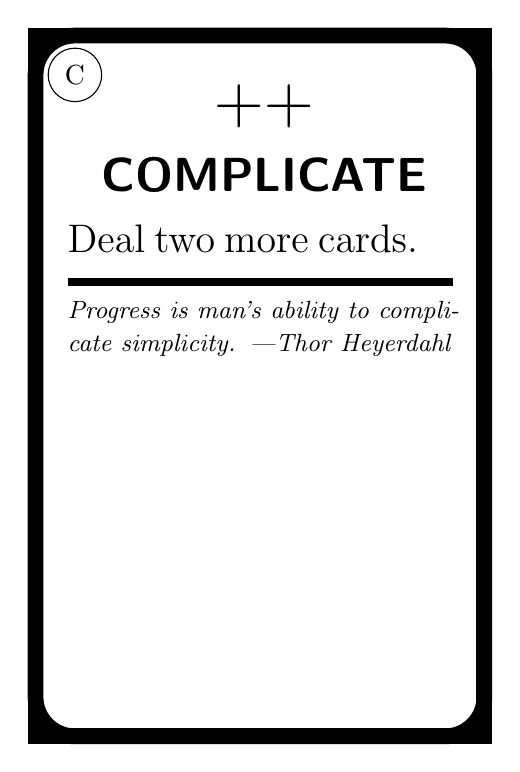
\begin{tikzpicture}
    \pgfmathsetmacro{\cardroundingradius}{5mm}
    \pgfmathsetmacro{\striproundingradius}{3mm}
    % \pgfmathsetmacro{\cardwidth}{5.9}
    % \pgfmathsetmacro{\cardheight}{9.2}
    \pgfmathsetmacro{\cardwidth}{5.7}
    \pgfmathsetmacro{\cardheight}{8.9}
    \pgfmathsetmacro{\stripwidth}{1.2}
    \pgfmathsetmacro{\strippadding}{0.1}
    \pgfmathsetmacro{\textpadding}{0.3}
    \pgfmathsetmacro{\ruleheight}{0.1}
    \providecommand{\stripfontsize}{\Huge}
    \providecommand{\captionfontsize}{\LARGE}
    \providecommand{\textfontsize}{\Large}
    \providecommand{\quotefontsize}{\small}
    \draw[line width=2mm,rounded corners=\cardroundingradius] (0,0) rectangle (\cardwidth,\cardheight);
    \draw[line width=2mm] (0,0) rectangle (\cardwidth,\cardheight);
    \node[text width=(\cardwidth-\strippadding-2*\textpadding)*1cm,below right,inner sep=0] at (\strippadding+\textpadding,\cardheight-\textpadding) 
    { 
    \begin{center} {\fontsize{80pt}{60pt}\selectfont ++}\\\end{center}
\begin{center}
    {\captionfontsize \textsf{\textbf{COMPLICATE}}}\end{center}
        {\textfontsize Deal two more cards.}\\
        \tikz{\fill (0,0) rectangle (\cardwidth-2*\strippadding-2*\textpadding,\ruleheight);}\\
        {\quotefontsize \textit{Progress is man's ability to complicate simplicity. ---Thor Heyerdahl}}\\[-2\baselineskip]
    };
    \node[circle,draw,text=black](c) at (.5,\cardheight-.5){C};
    \end{tikzpicture}%
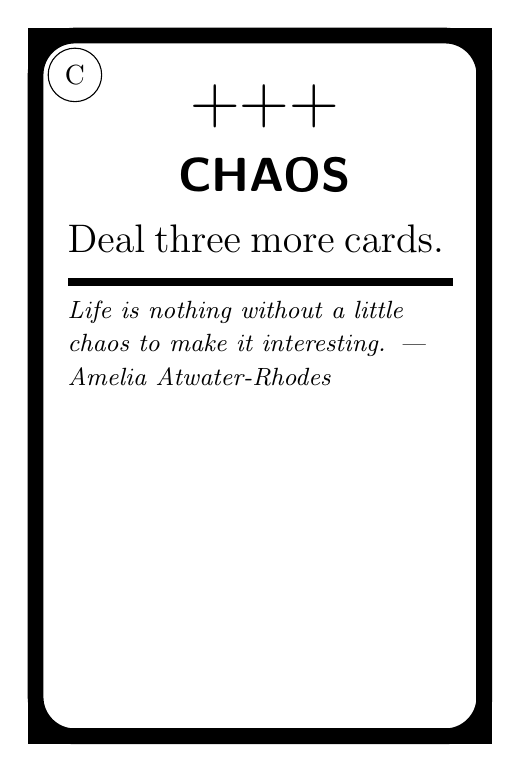
\begin{tikzpicture}
    \pgfmathsetmacro{\cardroundingradius}{5mm}
    \pgfmathsetmacro{\striproundingradius}{3mm}
    % \pgfmathsetmacro{\cardwidth}{5.9}
    % \pgfmathsetmacro{\cardheight}{9.2}
    \pgfmathsetmacro{\cardwidth}{5.7}
    \pgfmathsetmacro{\cardheight}{8.9}
    \pgfmathsetmacro{\stripwidth}{1.2}
    \pgfmathsetmacro{\strippadding}{0.1}
    \pgfmathsetmacro{\textpadding}{0.3}
    \pgfmathsetmacro{\ruleheight}{0.1}
    \providecommand{\stripfontsize}{\Huge}
    \providecommand{\captionfontsize}{\LARGE}
    \providecommand{\textfontsize}{\Large}
    \providecommand{\quotefontsize}{\small}
    \draw[line width=2mm,rounded corners=\cardroundingradius] (0,0) rectangle (\cardwidth,\cardheight);
    \draw[line width=2mm] (0,0) rectangle (\cardwidth,\cardheight);
    \node[text width=(\cardwidth-\strippadding-2*\textpadding)*1cm,below right,inner sep=0] at (\strippadding+\textpadding,\cardheight-\textpadding) 
    { 
    \begin{center} {\fontsize{80pt}{60pt}\selectfont +++}\\\end{center}
\begin{center}
    {\captionfontsize \textsf{\textbf{CHAOS}}}\end{center}
        {\textfontsize Deal three more cards.}\\
        \tikz{\fill (0,0) rectangle (\cardwidth-2*\strippadding-2*\textpadding,\ruleheight);}\\
        {\quotefontsize \textit{Life is nothing without a little chaos to make it interesting. ---Amelia Atwater-Rhodes}}\\[-2\baselineskip]
    };
    \node[circle,draw,text=black](c) at (.5,\cardheight-.5){C};
    \end{tikzpicture}%
\\[-\lineskip]
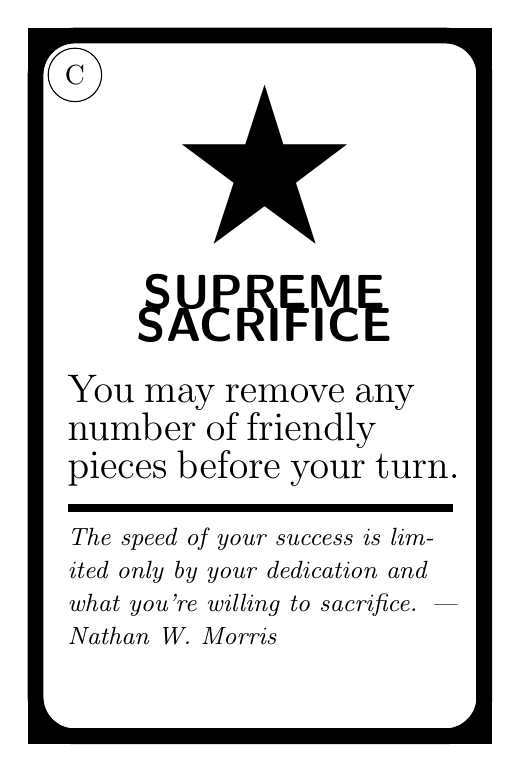
\begin{tikzpicture}
    \pgfmathsetmacro{\cardroundingradius}{5mm}
    \pgfmathsetmacro{\striproundingradius}{3mm}
    % \pgfmathsetmacro{\cardwidth}{5.9}
    % \pgfmathsetmacro{\cardheight}{9.2}
    \pgfmathsetmacro{\cardwidth}{5.7}
    \pgfmathsetmacro{\cardheight}{8.9}
    \pgfmathsetmacro{\stripwidth}{1.2}
    \pgfmathsetmacro{\strippadding}{0.1}
    \pgfmathsetmacro{\textpadding}{0.3}
    \pgfmathsetmacro{\ruleheight}{0.1}
    \providecommand{\stripfontsize}{\Huge}
    \providecommand{\captionfontsize}{\LARGE}
    \providecommand{\textfontsize}{\Large}
    \providecommand{\quotefontsize}{\small}
    \draw[line width=2mm,rounded corners=\cardroundingradius] (0,0) rectangle (\cardwidth,\cardheight);
    \draw[line width=2mm] (0,0) rectangle (\cardwidth,\cardheight);
    \node[text width=(\cardwidth-\strippadding-2*\textpadding)*1cm,below right,inner sep=0] at (\strippadding+\textpadding,\cardheight-\textpadding) 
    { 
    \begin{center} {\fontsize{80pt}{60pt}\selectfont \ding{72}}\\\end{center}
\begin{center}
    {\captionfontsize \textsf{\textbf{SUPREME SACRIFICE}}}\end{center}
        {\textfontsize You may remove any number of friendly pieces before your turn.}\\
        \tikz{\fill (0,0) rectangle (\cardwidth-2*\strippadding-2*\textpadding,\ruleheight);}\\
        {\quotefontsize \textit{The speed of your success is limited only by your dedication and what you're willing to sacrifice. ---Nathan W. Morris}}\\[-2\baselineskip]
    };
    \node[circle,draw,text=black](c) at (.5,\cardheight-.5){C};
    \end{tikzpicture}%
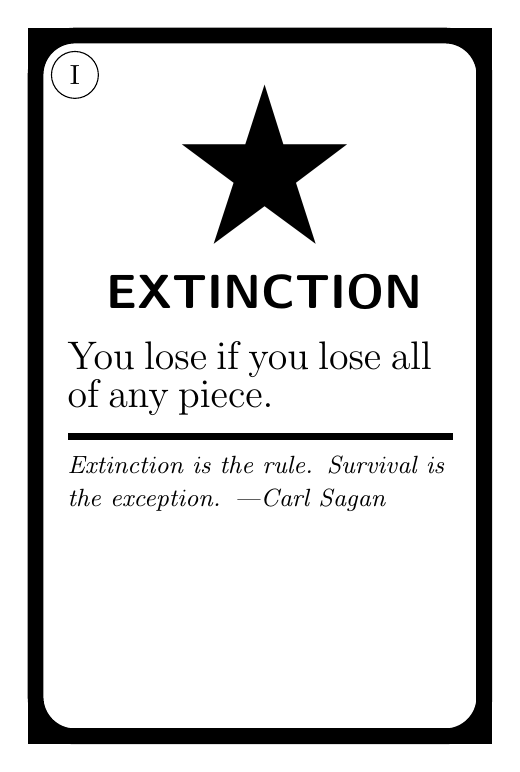
\begin{tikzpicture}
    \pgfmathsetmacro{\cardroundingradius}{5mm}
    \pgfmathsetmacro{\striproundingradius}{3mm}
    % \pgfmathsetmacro{\cardwidth}{5.9}
    % \pgfmathsetmacro{\cardheight}{9.2}
    \pgfmathsetmacro{\cardwidth}{5.7}
    \pgfmathsetmacro{\cardheight}{8.9}
    \pgfmathsetmacro{\stripwidth}{1.2}
    \pgfmathsetmacro{\strippadding}{0.1}
    \pgfmathsetmacro{\textpadding}{0.3}
    \pgfmathsetmacro{\ruleheight}{0.1}
    \providecommand{\stripfontsize}{\Huge}
    \providecommand{\captionfontsize}{\LARGE}
    \providecommand{\textfontsize}{\Large}
    \providecommand{\quotefontsize}{\small}
    \draw[line width=2mm,rounded corners=\cardroundingradius] (0,0) rectangle (\cardwidth,\cardheight);
    \draw[line width=2mm] (0,0) rectangle (\cardwidth,\cardheight);
    \node[text width=(\cardwidth-\strippadding-2*\textpadding)*1cm,below right,inner sep=0] at (\strippadding+\textpadding,\cardheight-\textpadding) 
    { 
    \begin{center} {\fontsize{80pt}{60pt}\selectfont \ding{72}}\\\end{center}
\begin{center}
    {\captionfontsize \textsf{\textbf{EXTINCTION}}}\end{center}
        {\textfontsize You lose if you lose all of any piece.}\\
        \tikz{\fill (0,0) rectangle (\cardwidth-2*\strippadding-2*\textpadding,\ruleheight);}\\
        {\quotefontsize \textit{Extinction is the rule. Survival is the exception. ---Carl Sagan}}\\[-2\baselineskip]
    };
    \node[circle,draw,text=black](c) at (.5,\cardheight-.5){I};
    \end{tikzpicture}%
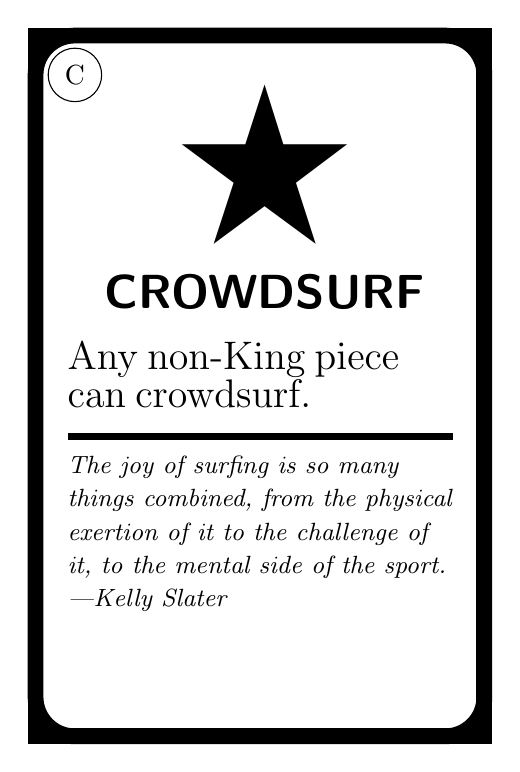
\begin{tikzpicture}
    \pgfmathsetmacro{\cardroundingradius}{5mm}
    \pgfmathsetmacro{\striproundingradius}{3mm}
    % \pgfmathsetmacro{\cardwidth}{5.9}
    % \pgfmathsetmacro{\cardheight}{9.2}
    \pgfmathsetmacro{\cardwidth}{5.7}
    \pgfmathsetmacro{\cardheight}{8.9}
    \pgfmathsetmacro{\stripwidth}{1.2}
    \pgfmathsetmacro{\strippadding}{0.1}
    \pgfmathsetmacro{\textpadding}{0.3}
    \pgfmathsetmacro{\ruleheight}{0.1}
    \providecommand{\stripfontsize}{\Huge}
    \providecommand{\captionfontsize}{\LARGE}
    \providecommand{\textfontsize}{\Large}
    \providecommand{\quotefontsize}{\small}
    \draw[line width=2mm,rounded corners=\cardroundingradius] (0,0) rectangle (\cardwidth,\cardheight);
    \draw[line width=2mm] (0,0) rectangle (\cardwidth,\cardheight);
    \node[text width=(\cardwidth-\strippadding-2*\textpadding)*1cm,below right,inner sep=0] at (\strippadding+\textpadding,\cardheight-\textpadding) 
    { 
    \begin{center} {\fontsize{80pt}{60pt}\selectfont \ding{72}}\\\end{center}
\begin{center}
    {\captionfontsize \textsf{\textbf{CROWDSURF}}}\end{center}
        {\textfontsize Any non-King piece can crowdsurf.}\\
        \tikz{\fill (0,0) rectangle (\cardwidth-2*\strippadding-2*\textpadding,\ruleheight);}\\
        {\quotefontsize \textit{The joy of surfing is so many things combined, from the physical exertion of it to the challenge of it, to the mental side of the sport. ---Kelly Slater}}\\[-2\baselineskip]
    };
    \node[circle,draw,text=black](c) at (.5,\cardheight-.5){C};
    \end{tikzpicture}%
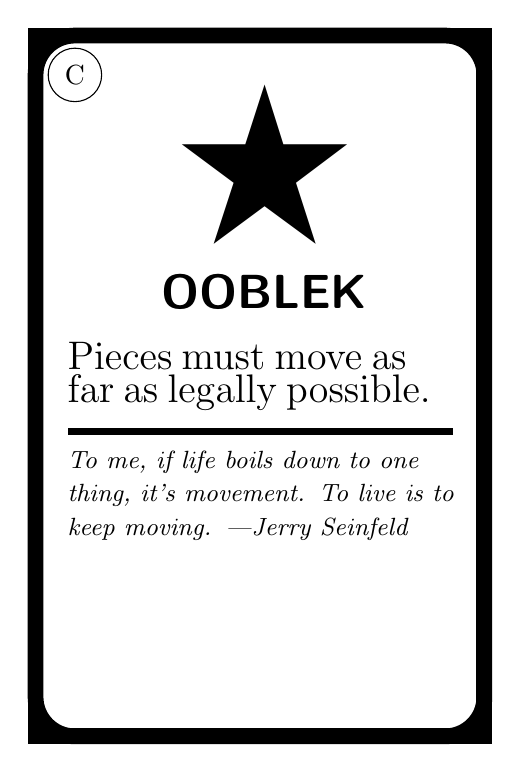
\begin{tikzpicture}
    \pgfmathsetmacro{\cardroundingradius}{5mm}
    \pgfmathsetmacro{\striproundingradius}{3mm}
    % \pgfmathsetmacro{\cardwidth}{5.9}
    % \pgfmathsetmacro{\cardheight}{9.2}
    \pgfmathsetmacro{\cardwidth}{5.7}
    \pgfmathsetmacro{\cardheight}{8.9}
    \pgfmathsetmacro{\stripwidth}{1.2}
    \pgfmathsetmacro{\strippadding}{0.1}
    \pgfmathsetmacro{\textpadding}{0.3}
    \pgfmathsetmacro{\ruleheight}{0.1}
    \providecommand{\stripfontsize}{\Huge}
    \providecommand{\captionfontsize}{\LARGE}
    \providecommand{\textfontsize}{\Large}
    \providecommand{\quotefontsize}{\small}
    \draw[line width=2mm,rounded corners=\cardroundingradius] (0,0) rectangle (\cardwidth,\cardheight);
    \draw[line width=2mm] (0,0) rectangle (\cardwidth,\cardheight);
    \node[text width=(\cardwidth-\strippadding-2*\textpadding)*1cm,below right,inner sep=0] at (\strippadding+\textpadding,\cardheight-\textpadding) 
    { 
    \begin{center} {\fontsize{80pt}{60pt}\selectfont \ding{72}}\\\end{center}
\begin{center}
    {\captionfontsize \textsf{\textbf{OOBLEK}}}\end{center}
        {\textfontsize Pieces must move as far as legally possible.}\\
        \tikz{\fill (0,0) rectangle (\cardwidth-2*\strippadding-2*\textpadding,\ruleheight);}\\
        {\quotefontsize \textit{To me, if life boils down to one thing, it's movement. To live is to keep moving. ---Jerry Seinfeld}}\\[-2\baselineskip]
    };
    \node[circle,draw,text=black](c) at (.5,\cardheight-.5){C};
    \end{tikzpicture}%
\\[-\lineskip]
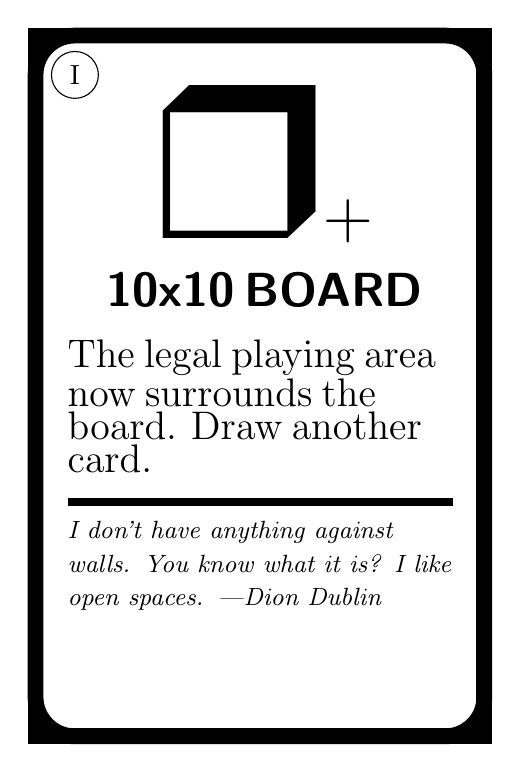
\begin{tikzpicture}
    \pgfmathsetmacro{\cardroundingradius}{5mm}
    \pgfmathsetmacro{\striproundingradius}{3mm}
    % \pgfmathsetmacro{\cardwidth}{5.9}
    % \pgfmathsetmacro{\cardheight}{9.2}
    \pgfmathsetmacro{\cardwidth}{5.7}
    \pgfmathsetmacro{\cardheight}{8.9}
    \pgfmathsetmacro{\stripwidth}{1.2}
    \pgfmathsetmacro{\strippadding}{0.1}
    \pgfmathsetmacro{\textpadding}{0.3}
    \pgfmathsetmacro{\ruleheight}{0.1}
    \providecommand{\stripfontsize}{\Huge}
    \providecommand{\captionfontsize}{\LARGE}
    \providecommand{\textfontsize}{\Large}
    \providecommand{\quotefontsize}{\small}
    \draw[line width=2mm,rounded corners=\cardroundingradius] (0,0) rectangle (\cardwidth,\cardheight);
    \draw[line width=2mm] (0,0) rectangle (\cardwidth,\cardheight);
    \node[text width=(\cardwidth-\strippadding-2*\textpadding)*1cm,below right,inner sep=0] at (\strippadding+\textpadding,\cardheight-\textpadding) 
    { 
    \begin{center} {\fontsize{80pt}{60pt}\selectfont \ding{114}+}\\\end{center}
\begin{center}
    {\captionfontsize \textsf{\textbf{10x10 BOARD}}}\end{center}
        {\textfontsize The legal playing area now surrounds the board. Draw another card.}\\
        \tikz{\fill (0,0) rectangle (\cardwidth-2*\strippadding-2*\textpadding,\ruleheight);}\\
        {\quotefontsize \textit{I don't have anything against walls. You know what it is? I like open spaces. ---Dion Dublin}}\\[-2\baselineskip]
    };
    \node[circle,draw,text=black](c) at (.5,\cardheight-.5){I};
    \end{tikzpicture}%
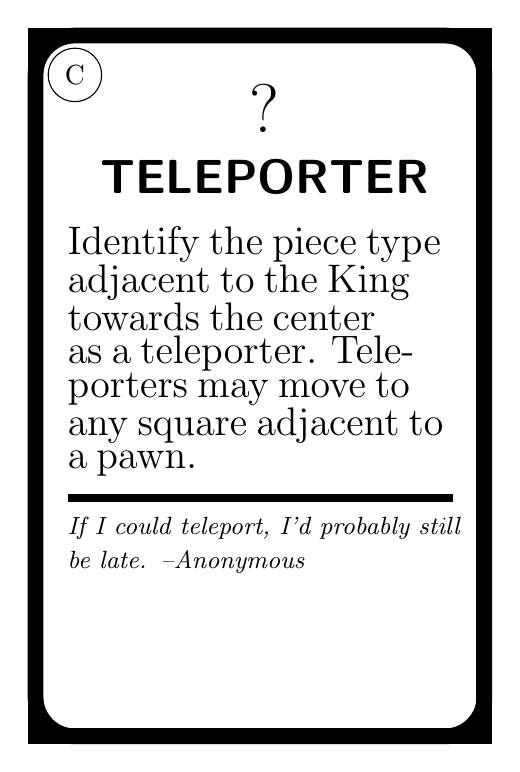
\begin{tikzpicture}
    \pgfmathsetmacro{\cardroundingradius}{5mm}
    \pgfmathsetmacro{\striproundingradius}{3mm}
    % \pgfmathsetmacro{\cardwidth}{5.9}
    % \pgfmathsetmacro{\cardheight}{9.2}
    \pgfmathsetmacro{\cardwidth}{5.7}
    \pgfmathsetmacro{\cardheight}{8.9}
    \pgfmathsetmacro{\stripwidth}{1.2}
    \pgfmathsetmacro{\strippadding}{0.1}
    \pgfmathsetmacro{\textpadding}{0.3}
    \pgfmathsetmacro{\ruleheight}{0.1}
    \providecommand{\stripfontsize}{\Huge}
    \providecommand{\captionfontsize}{\LARGE}
    \providecommand{\textfontsize}{\Large}
    \providecommand{\quotefontsize}{\small}
    \draw[line width=2mm,rounded corners=\cardroundingradius] (0,0) rectangle (\cardwidth,\cardheight);
    \draw[line width=2mm] (0,0) rectangle (\cardwidth,\cardheight);
    \node[text width=(\cardwidth-\strippadding-2*\textpadding)*1cm,below right,inner sep=0] at (\strippadding+\textpadding,\cardheight-\textpadding) 
    { 
    \begin{center} {\fontsize{80pt}{60pt}\selectfont ?}\\\end{center}
\begin{center}
    {\captionfontsize \textsf{\textbf{TELEPORTER}}}\end{center}
        {\textfontsize Identify the piece type adjacent to the King towards the center as a teleporter. Teleporters may move to any square adjacent to a pawn.}\\
        \tikz{\fill (0,0) rectangle (\cardwidth-2*\strippadding-2*\textpadding,\ruleheight);}\\
        {\quotefontsize \textit{If I could teleport, I'd probably still be late. --Anonymous}}\\[-2\baselineskip]
    };
    \node[circle,draw,text=black](c) at (.5,\cardheight-.5){C};
    \end{tikzpicture}%
\begin{tikzpicture}
    \pgfmathsetmacro{\cardroundingradius}{5mm}
    \pgfmathsetmacro{\striproundingradius}{3mm}
    % \pgfmathsetmacro{\cardwidth}{5.9}
    % \pgfmathsetmacro{\cardheight}{9.2}
    \pgfmathsetmacro{\cardwidth}{5.7}
    \pgfmathsetmacro{\cardheight}{8.9}
    \pgfmathsetmacro{\stripwidth}{1.2}
    \pgfmathsetmacro{\strippadding}{0.1}
    \pgfmathsetmacro{\textpadding}{0.3}
    \pgfmathsetmacro{\ruleheight}{0.1}
    \providecommand{\stripfontsize}{\Huge}
    \providecommand{\captionfontsize}{\LARGE}
    \providecommand{\textfontsize}{\Large}
    \providecommand{\quotefontsize}{\small}
    \draw[line width=2mm,rounded corners=\cardroundingradius] (0,0) rectangle (\cardwidth,\cardheight);
    \draw[line width=2mm] (0,0) rectangle (\cardwidth,\cardheight);
    \node[text width=(\cardwidth-\strippadding-2*\textpadding)*1cm,below right,inner sep=0] at (\strippadding+\textpadding,\cardheight-\textpadding) 
    { 
    \begin{center} {\fontsize{80pt}{60pt}\selectfont ♘♗}\\\end{center}
\begin{center}
    {\captionfontsize \textsf{\textbf{MINOR TENET}}}\end{center}
        {\textfontsize Bishops move and take backwards like Knights. Knights move and take backward like Bishops.}\\
        \tikz{\fill (0,0) rectangle (\cardwidth-2*\strippadding-2*\textpadding,\ruleheight);}\\
        {\quotefontsize \textit{Bold I'm Fine With. I Thought You Were Gonna Say Nuts. ---Mahir}}\\[-2\baselineskip]
    };
    \node[circle,draw,text=black](c) at (.5,\cardheight-.5){C};
    \end{tikzpicture}%
\begin{tikzpicture}
    \pgfmathsetmacro{\cardroundingradius}{5mm}
    \pgfmathsetmacro{\striproundingradius}{3mm}
    % \pgfmathsetmacro{\cardwidth}{5.9}
    % \pgfmathsetmacro{\cardheight}{9.2}
    \pgfmathsetmacro{\cardwidth}{5.7}
    \pgfmathsetmacro{\cardheight}{8.9}
    \pgfmathsetmacro{\stripwidth}{1.2}
    \pgfmathsetmacro{\strippadding}{0.1}
    \pgfmathsetmacro{\textpadding}{0.3}
    \pgfmathsetmacro{\ruleheight}{0.1}
    \providecommand{\stripfontsize}{\Huge}
    \providecommand{\captionfontsize}{\LARGE}
    \providecommand{\textfontsize}{\Large}
    \providecommand{\quotefontsize}{\small}
    \draw[line width=2mm,rounded corners=\cardroundingradius] (0,0) rectangle (\cardwidth,\cardheight);
    \draw[line width=2mm] (0,0) rectangle (\cardwidth,\cardheight);
    \node[text width=(\cardwidth-\strippadding-2*\textpadding)*1cm,below right,inner sep=0] at (\strippadding+\textpadding,\cardheight-\textpadding) 
    { 
    \begin{center} {\fontsize{80pt}{60pt}\selectfont ♕}\\\end{center}
\begin{center}
    {\captionfontsize \textsf{\textbf{NIGHT KING QUEEN}}}\end{center}
        {\textfontsize Queens move and take like Knight+King.}\\
        \tikz{\fill (0,0) rectangle (\cardwidth-2*\strippadding-2*\textpadding,\ruleheight);}\\
        {\quotefontsize \textit{Night's King was only a man by light of day, Old Nan would always say, but the night was his to rule. ---Brandon Stark}}\\[-2\baselineskip]
    };
    \node[circle,draw,text=black](c) at (.5,\cardheight-.5){?};
    \end{tikzpicture}%
\\[-\lineskip]
\begin{tikzpicture}
    \pgfmathsetmacro{\cardroundingradius}{5mm}
    \pgfmathsetmacro{\striproundingradius}{3mm}
    % \pgfmathsetmacro{\cardwidth}{5.9}
    % \pgfmathsetmacro{\cardheight}{9.2}
    \pgfmathsetmacro{\cardwidth}{5.7}
    \pgfmathsetmacro{\cardheight}{8.9}
    \pgfmathsetmacro{\stripwidth}{1.2}
    \pgfmathsetmacro{\strippadding}{0.1}
    \pgfmathsetmacro{\textpadding}{0.3}
    \pgfmathsetmacro{\ruleheight}{0.1}
    \providecommand{\stripfontsize}{\Huge}
    \providecommand{\captionfontsize}{\LARGE}
    \providecommand{\textfontsize}{\Large}
    \providecommand{\quotefontsize}{\small}
    \draw[line width=2mm,rounded corners=\cardroundingradius] (0,0) rectangle (\cardwidth,\cardheight);
    \draw[line width=2mm] (0,0) rectangle (\cardwidth,\cardheight);
    \node[text width=(\cardwidth-\strippadding-2*\textpadding)*1cm,below right,inner sep=0] at (\strippadding+\textpadding,\cardheight-\textpadding) 
    { 
    \begin{center} {\fontsize{80pt}{60pt}\selectfont ♕}\\\end{center}
\begin{center}
    {\captionfontsize \textsf{\textbf{ARCHBISHOP}}}\end{center}
        {\textfontsize Queens move and take like Bishop+Knight. Fairy chess Archbishop.}\\
        \tikz{\fill (0,0) rectangle (\cardwidth-2*\strippadding-2*\textpadding,\ruleheight);}\\
        {\quotefontsize \textit{If people want a sense of purpose they should get it from their archbishop. They should certainly not get it from their politicians. ---Harold MacMillan}}\\[-2\baselineskip]
    };
    \node[circle,draw,text=black](c) at (.5,\cardheight-.5){F};
    \end{tikzpicture}%
\begin{tikzpicture}
    \pgfmathsetmacro{\cardroundingradius}{5mm}
    \pgfmathsetmacro{\striproundingradius}{3mm}
    % \pgfmathsetmacro{\cardwidth}{5.9}
    % \pgfmathsetmacro{\cardheight}{9.2}
    \pgfmathsetmacro{\cardwidth}{5.7}
    \pgfmathsetmacro{\cardheight}{8.9}
    \pgfmathsetmacro{\stripwidth}{1.2}
    \pgfmathsetmacro{\strippadding}{0.1}
    \pgfmathsetmacro{\textpadding}{0.3}
    \pgfmathsetmacro{\ruleheight}{0.1}
    \providecommand{\stripfontsize}{\Huge}
    \providecommand{\captionfontsize}{\LARGE}
    \providecommand{\textfontsize}{\Large}
    \providecommand{\quotefontsize}{\small}
    \draw[line width=2mm,rounded corners=\cardroundingradius] (0,0) rectangle (\cardwidth,\cardheight);
    \draw[line width=2mm] (0,0) rectangle (\cardwidth,\cardheight);
    \node[text width=(\cardwidth-\strippadding-2*\textpadding)*1cm,below right,inner sep=0] at (\strippadding+\textpadding,\cardheight-\textpadding) 
    { 
    \begin{center} {\fontsize{80pt}{60pt}\selectfont ♕}\\\end{center}
\begin{center}
    {\captionfontsize \textsf{\textbf{CHANCELLOR}}}\end{center}
        {\textfontsize Queens move and take like Rook+Knight. Fairy chess Chancellor.}\\
        \tikz{\fill (0,0) rectangle (\cardwidth-2*\strippadding-2*\textpadding,\ruleheight);}\\
        {\quotefontsize \textit{When I'm stirring a saucepan, I don't say to myself, 'Now the chancellor is stirring a saucepan'. ---Angela Merkel}}\\[-2\baselineskip]
    };
    \node[circle,draw,text=black](c) at (.5,\cardheight-.5){F};
    \end{tikzpicture}%
\begin{tikzpicture}
    \pgfmathsetmacro{\cardroundingradius}{5mm}
    \pgfmathsetmacro{\striproundingradius}{3mm}
    % \pgfmathsetmacro{\cardwidth}{5.9}
    % \pgfmathsetmacro{\cardheight}{9.2}
    \pgfmathsetmacro{\cardwidth}{5.7}
    \pgfmathsetmacro{\cardheight}{8.9}
    \pgfmathsetmacro{\stripwidth}{1.2}
    \pgfmathsetmacro{\strippadding}{0.1}
    \pgfmathsetmacro{\textpadding}{0.3}
    \pgfmathsetmacro{\ruleheight}{0.1}
    \providecommand{\stripfontsize}{\Huge}
    \providecommand{\captionfontsize}{\LARGE}
    \providecommand{\textfontsize}{\Large}
    \providecommand{\quotefontsize}{\small}
    \draw[line width=2mm,rounded corners=\cardroundingradius] (0,0) rectangle (\cardwidth,\cardheight);
    \draw[line width=2mm] (0,0) rectangle (\cardwidth,\cardheight);
    \node[text width=(\cardwidth-\strippadding-2*\textpadding)*1cm,below right,inner sep=0] at (\strippadding+\textpadding,\cardheight-\textpadding) 
    { 
    \begin{center} {\fontsize{80pt}{60pt}\selectfont ♖+}\\\end{center}
\begin{center}
    {\captionfontsize \textsf{\textbf{BLOCKADE}}}\end{center}
        {\textfontsize At the end of a Rook move, it may be inverted. Upside-down rooks cannot be taken or attack.}\\
        \tikz{\fill (0,0) rectangle (\cardwidth-2*\strippadding-2*\textpadding,\ruleheight);}\\
        {\quotefontsize \textit{Everyone thinks at some point if what they are doing has any meaning or not. ---William Macbeth}}\\[-2\baselineskip]
    };
    \node[circle,draw,text=black](c) at (.5,\cardheight-.5){C};
    \end{tikzpicture}%
\begin{tikzpicture}
    \pgfmathsetmacro{\cardroundingradius}{5mm}
    \pgfmathsetmacro{\striproundingradius}{3mm}
    % \pgfmathsetmacro{\cardwidth}{5.9}
    % \pgfmathsetmacro{\cardheight}{9.2}
    \pgfmathsetmacro{\cardwidth}{5.7}
    \pgfmathsetmacro{\cardheight}{8.9}
    \pgfmathsetmacro{\stripwidth}{1.2}
    \pgfmathsetmacro{\strippadding}{0.1}
    \pgfmathsetmacro{\textpadding}{0.3}
    \pgfmathsetmacro{\ruleheight}{0.1}
    \providecommand{\stripfontsize}{\Huge}
    \providecommand{\captionfontsize}{\LARGE}
    \providecommand{\textfontsize}{\Large}
    \providecommand{\quotefontsize}{\small}
    \draw[line width=2mm,rounded corners=\cardroundingradius] (0,0) rectangle (\cardwidth,\cardheight);
    \draw[line width=2mm] (0,0) rectangle (\cardwidth,\cardheight);
    \node[text width=(\cardwidth-\strippadding-2*\textpadding)*1cm,below right,inner sep=0] at (\strippadding+\textpadding,\cardheight-\textpadding) 
    { 
    \begin{center} {\fontsize{80pt}{60pt}\selectfont ♖}\\\end{center}
\begin{center}
    {\captionfontsize \textsf{\textbf{CHINESE CANNON}}}\end{center}
        {\textfontsize A rook takes by throwing a friendly piece so that it jumps the rook in a rook direction.}\\
        \tikz{\fill (0,0) rectangle (\cardwidth-2*\strippadding-2*\textpadding,\ruleheight);}\\
        {\quotefontsize \textit{I spend most of my life feeling like I've been shot out of a cannon. ---Molly Ivins}}\\[-2\baselineskip]
    };
    \node[circle,draw,text=black](c) at (.5,\cardheight-.5){?};
    \end{tikzpicture}%
\\[-\lineskip]
\begin{tikzpicture}
    \pgfmathsetmacro{\cardroundingradius}{5mm}
    \pgfmathsetmacro{\striproundingradius}{3mm}
    % \pgfmathsetmacro{\cardwidth}{5.9}
    % \pgfmathsetmacro{\cardheight}{9.2}
    \pgfmathsetmacro{\cardwidth}{5.7}
    \pgfmathsetmacro{\cardheight}{8.9}
    \pgfmathsetmacro{\stripwidth}{1.2}
    \pgfmathsetmacro{\strippadding}{0.1}
    \pgfmathsetmacro{\textpadding}{0.3}
    \pgfmathsetmacro{\ruleheight}{0.1}
    \providecommand{\stripfontsize}{\Huge}
    \providecommand{\captionfontsize}{\LARGE}
    \providecommand{\textfontsize}{\Large}
    \providecommand{\quotefontsize}{\small}
    \draw[line width=2mm,rounded corners=\cardroundingradius] (0,0) rectangle (\cardwidth,\cardheight);
    \draw[line width=2mm] (0,0) rectangle (\cardwidth,\cardheight);
    \node[text width=(\cardwidth-\strippadding-2*\textpadding)*1cm,below right,inner sep=0] at (\strippadding+\textpadding,\cardheight-\textpadding) 
    { 
    \begin{center} {\fontsize{80pt}{60pt}\selectfont ♖}\\\end{center}
\begin{center}
    {\captionfontsize \textsf{\textbf{IMMOBILIZER}}}\end{center}
        {\textfontsize Pieces adjacent to an enemy Rook may not move. Rooks may not capture.}\\
        \tikz{\fill (0,0) rectangle (\cardwidth-2*\strippadding-2*\textpadding,\ruleheight);}\\
        {\quotefontsize \textit{The activity of worrying keeps you immobilized. ---Wayne Dyer}}\\[-2\baselineskip]
    };
    \node[circle,draw,text=black](c) at (.5,\cardheight-.5){U};
    \end{tikzpicture}%
\begin{tikzpicture}
    \pgfmathsetmacro{\cardroundingradius}{5mm}
    \pgfmathsetmacro{\striproundingradius}{3mm}
    % \pgfmathsetmacro{\cardwidth}{5.9}
    % \pgfmathsetmacro{\cardheight}{9.2}
    \pgfmathsetmacro{\cardwidth}{5.7}
    \pgfmathsetmacro{\cardheight}{8.9}
    \pgfmathsetmacro{\stripwidth}{1.2}
    \pgfmathsetmacro{\strippadding}{0.1}
    \pgfmathsetmacro{\textpadding}{0.3}
    \pgfmathsetmacro{\ruleheight}{0.1}
    \providecommand{\stripfontsize}{\Huge}
    \providecommand{\captionfontsize}{\LARGE}
    \providecommand{\textfontsize}{\Large}
    \providecommand{\quotefontsize}{\small}
    \draw[line width=2mm,rounded corners=\cardroundingradius] (0,0) rectangle (\cardwidth,\cardheight);
    \draw[line width=2mm] (0,0) rectangle (\cardwidth,\cardheight);
    \node[text width=(\cardwidth-\strippadding-2*\textpadding)*1cm,below right,inner sep=0] at (\strippadding+\textpadding,\cardheight-\textpadding) 
    { 
    \begin{center} {\fontsize{80pt}{60pt}\selectfont ♖♗}\\\end{center}
\begin{center}
    {\captionfontsize \textsf{\textbf{ROYAL REVERSE}}}\end{center}
        {\textfontsize Bishops and Rooks may move and take backwards like a Queen.}\\
        \tikz{\fill (0,0) rectangle (\cardwidth-2*\strippadding-2*\textpadding,\ruleheight);}\\
        {\quotefontsize \textit{To the royal guards of this realm, we are all victims in-waiting. ---Cheshire Cat}}\\[-2\baselineskip]
    };
    \node[circle,draw,text=black](c) at (.5,\cardheight-.5){C};
    \end{tikzpicture}%
\begin{tikzpicture}
    \pgfmathsetmacro{\cardroundingradius}{5mm}
    \pgfmathsetmacro{\striproundingradius}{3mm}
    % \pgfmathsetmacro{\cardwidth}{5.9}
    % \pgfmathsetmacro{\cardheight}{9.2}
    \pgfmathsetmacro{\cardwidth}{5.7}
    \pgfmathsetmacro{\cardheight}{8.9}
    \pgfmathsetmacro{\stripwidth}{1.2}
    \pgfmathsetmacro{\strippadding}{0.1}
    \pgfmathsetmacro{\textpadding}{0.3}
    \pgfmathsetmacro{\ruleheight}{0.1}
    \providecommand{\stripfontsize}{\Huge}
    \providecommand{\captionfontsize}{\LARGE}
    \providecommand{\textfontsize}{\Large}
    \providecommand{\quotefontsize}{\small}
    \draw[line width=2mm,rounded corners=\cardroundingradius] (0,0) rectangle (\cardwidth,\cardheight);
    \draw[line width=2mm] (0,0) rectangle (\cardwidth,\cardheight);
    \node[text width=(\cardwidth-\strippadding-2*\textpadding)*1cm,below right,inner sep=0] at (\strippadding+\textpadding,\cardheight-\textpadding) 
    { 
    \begin{center} {\fontsize{80pt}{60pt}\selectfont ♖♕}\\\end{center}
\begin{center}
    {\captionfontsize \textsf{\textbf{ROOK-QUEEN SWAP}}}\end{center}
        {\textfontsize Queens and Rooks move normally, but take like each other.}\\
        \tikz{\fill (0,0) rectangle (\cardwidth-2*\strippadding-2*\textpadding,\ruleheight);}\\
        {\quotefontsize \textit{I am definitely the queen. I definitely see myself as the queen. ---Lil' Kim}}\\[-2\baselineskip]
    };
    \node[circle,draw,text=black](c) at (.5,\cardheight-.5){?};
    \end{tikzpicture}%
\begin{tikzpicture}
    \pgfmathsetmacro{\cardroundingradius}{5mm}
    \pgfmathsetmacro{\striproundingradius}{3mm}
    % \pgfmathsetmacro{\cardwidth}{5.9}
    % \pgfmathsetmacro{\cardheight}{9.2}
    \pgfmathsetmacro{\cardwidth}{5.7}
    \pgfmathsetmacro{\cardheight}{8.9}
    \pgfmathsetmacro{\stripwidth}{1.2}
    \pgfmathsetmacro{\strippadding}{0.1}
    \pgfmathsetmacro{\textpadding}{0.3}
    \pgfmathsetmacro{\ruleheight}{0.1}
    \providecommand{\stripfontsize}{\Huge}
    \providecommand{\captionfontsize}{\LARGE}
    \providecommand{\textfontsize}{\Large}
    \providecommand{\quotefontsize}{\small}
    \draw[line width=2mm,rounded corners=\cardroundingradius] (0,0) rectangle (\cardwidth,\cardheight);
    \draw[line width=2mm] (0,0) rectangle (\cardwidth,\cardheight);
    \node[text width=(\cardwidth-\strippadding-2*\textpadding)*1cm,below right,inner sep=0] at (\strippadding+\textpadding,\cardheight-\textpadding) 
    { 
    \begin{center} {\fontsize{80pt}{60pt}\selectfont ♘♔}\\\end{center}
\begin{center}
    {\captionfontsize \textsf{\textbf{KNIGHT-KING SWAP}}}\end{center}
        {\textfontsize Knights and Kings move/take like each other.}\\
        \tikz{\fill (0,0) rectangle (\cardwidth-2*\strippadding-2*\textpadding,\ruleheight);}\\
        {\quotefontsize \textit{If I was King for just one day, I would give it all away. --Thompson Twins}}\\[-2\baselineskip]
    };
    \node[circle,draw,text=black](c) at (.5,\cardheight-.5){I};
    \end{tikzpicture}%
\\[-\lineskip]
\begin{tikzpicture}
    \pgfmathsetmacro{\cardroundingradius}{5mm}
    \pgfmathsetmacro{\striproundingradius}{3mm}
    % \pgfmathsetmacro{\cardwidth}{5.9}
    % \pgfmathsetmacro{\cardheight}{9.2}
    \pgfmathsetmacro{\cardwidth}{5.7}
    \pgfmathsetmacro{\cardheight}{8.9}
    \pgfmathsetmacro{\stripwidth}{1.2}
    \pgfmathsetmacro{\strippadding}{0.1}
    \pgfmathsetmacro{\textpadding}{0.3}
    \pgfmathsetmacro{\ruleheight}{0.1}
    \providecommand{\stripfontsize}{\Huge}
    \providecommand{\captionfontsize}{\LARGE}
    \providecommand{\textfontsize}{\Large}
    \providecommand{\quotefontsize}{\small}
    \draw[line width=2mm,rounded corners=\cardroundingradius] (0,0) rectangle (\cardwidth,\cardheight);
    \draw[line width=2mm] (0,0) rectangle (\cardwidth,\cardheight);
    \node[text width=(\cardwidth-\strippadding-2*\textpadding)*1cm,below right,inner sep=0] at (\strippadding+\textpadding,\cardheight-\textpadding) 
    { 
    \begin{center} {\fontsize{80pt}{60pt}\selectfont ♔}\\\end{center}
\begin{center}
    {\captionfontsize \textsf{\textbf{KING CHAMELEON}}}\end{center}
        {\textfontsize Kings may also move/take like any piece attacking them.}\\
        \tikz{\fill (0,0) rectangle (\cardwidth-2*\strippadding-2*\textpadding,\ruleheight);}\\
        {\quotefontsize \textit{I can kind of be a chameleon. ---Sasha Spielberg}}\\[-2\baselineskip]
    };
    \node[circle,draw,text=black](c) at (.5,\cardheight-.5){I};
    \end{tikzpicture}%
\begin{tikzpicture}
    \pgfmathsetmacro{\cardroundingradius}{5mm}
    \pgfmathsetmacro{\striproundingradius}{3mm}
    % \pgfmathsetmacro{\cardwidth}{5.9}
    % \pgfmathsetmacro{\cardheight}{9.2}
    \pgfmathsetmacro{\cardwidth}{5.7}
    \pgfmathsetmacro{\cardheight}{8.9}
    \pgfmathsetmacro{\stripwidth}{1.2}
    \pgfmathsetmacro{\strippadding}{0.1}
    \pgfmathsetmacro{\textpadding}{0.3}
    \pgfmathsetmacro{\ruleheight}{0.1}
    \providecommand{\stripfontsize}{\Huge}
    \providecommand{\captionfontsize}{\LARGE}
    \providecommand{\textfontsize}{\Large}
    \providecommand{\quotefontsize}{\small}
    \draw[line width=2mm,rounded corners=\cardroundingradius] (0,0) rectangle (\cardwidth,\cardheight);
    \draw[line width=2mm] (0,0) rectangle (\cardwidth,\cardheight);
    \node[text width=(\cardwidth-\strippadding-2*\textpadding)*1cm,below right,inner sep=0] at (\strippadding+\textpadding,\cardheight-\textpadding) 
    { 
    \begin{center} {\fontsize{80pt}{60pt}\selectfont ♗}\\\end{center}
\begin{center}
    {\captionfontsize \textsf{\textbf{SUMMONER}}}\end{center}
        {\textfontsize Bishops may summon a friendly non-King piece to an adjacent square}\\
        \tikz{\fill (0,0) rectangle (\cardwidth-2*\strippadding-2*\textpadding,\ruleheight);}\\
        {\quotefontsize \textit{My name is Mortimer Alexander and I am a licensed summoner." "Darn. I'd hoped you were the pizza delivery guy. ---Jana Oliver}}\\[-2\baselineskip]
    };
    \node[circle,draw,text=black](c) at (.5,\cardheight-.5){?};
    \end{tikzpicture}%
\begin{tikzpicture}
    \pgfmathsetmacro{\cardroundingradius}{5mm}
    \pgfmathsetmacro{\striproundingradius}{3mm}
    % \pgfmathsetmacro{\cardwidth}{5.9}
    % \pgfmathsetmacro{\cardheight}{9.2}
    \pgfmathsetmacro{\cardwidth}{5.7}
    \pgfmathsetmacro{\cardheight}{8.9}
    \pgfmathsetmacro{\stripwidth}{1.2}
    \pgfmathsetmacro{\strippadding}{0.1}
    \pgfmathsetmacro{\textpadding}{0.3}
    \pgfmathsetmacro{\ruleheight}{0.1}
    \providecommand{\stripfontsize}{\Huge}
    \providecommand{\captionfontsize}{\LARGE}
    \providecommand{\textfontsize}{\Large}
    \providecommand{\quotefontsize}{\small}
    \draw[line width=2mm,rounded corners=\cardroundingradius] (0,0) rectangle (\cardwidth,\cardheight);
    \draw[line width=2mm] (0,0) rectangle (\cardwidth,\cardheight);
    \node[text width=(\cardwidth-\strippadding-2*\textpadding)*1cm,below right,inner sep=0] at (\strippadding+\textpadding,\cardheight-\textpadding) 
    { 
    \begin{center} {\fontsize{80pt}{60pt}\selectfont ♗}\\\end{center}
\begin{center}
    {\captionfontsize \textsf{\textbf{BISHOP CHAMPION}}}\end{center}
        {\textfontsize Bishops may move/take using a 2 square jump in any direction. They may also move/take one square rectilinearly.}\\
        \tikz{\fill (0,0) rectangle (\cardwidth-2*\strippadding-2*\textpadding,\ruleheight);}\\
        {\quotefontsize \textit{Every absurdity has a champion to defend it. ---Oliver Goldsmith}}\\[-2\baselineskip]
    };
    \node[circle,draw,text=black](c) at (.5,\cardheight-.5){Ω};
    \end{tikzpicture}%
\begin{tikzpicture}
    \pgfmathsetmacro{\cardroundingradius}{5mm}
    \pgfmathsetmacro{\striproundingradius}{3mm}
    % \pgfmathsetmacro{\cardwidth}{5.9}
    % \pgfmathsetmacro{\cardheight}{9.2}
    \pgfmathsetmacro{\cardwidth}{5.7}
    \pgfmathsetmacro{\cardheight}{8.9}
    \pgfmathsetmacro{\stripwidth}{1.2}
    \pgfmathsetmacro{\strippadding}{0.1}
    \pgfmathsetmacro{\textpadding}{0.3}
    \pgfmathsetmacro{\ruleheight}{0.1}
    \providecommand{\stripfontsize}{\Huge}
    \providecommand{\captionfontsize}{\LARGE}
    \providecommand{\textfontsize}{\Large}
    \providecommand{\quotefontsize}{\small}
    \draw[line width=2mm,rounded corners=\cardroundingradius] (0,0) rectangle (\cardwidth,\cardheight);
    \draw[line width=2mm] (0,0) rectangle (\cardwidth,\cardheight);
    \node[text width=(\cardwidth-\strippadding-2*\textpadding)*1cm,below right,inner sep=0] at (\strippadding+\textpadding,\cardheight-\textpadding) 
    { 
    \begin{center} {\fontsize{80pt}{60pt}\selectfont ♗}\\\end{center}
\begin{center}
    {\captionfontsize \textsf{\textbf{RETREATER}}}\end{center}
        {\textfontsize Bishops move like a queen, but take by moving away from an adjacent piece.}\\
        \tikz{\fill (0,0) rectangle (\cardwidth-2*\strippadding-2*\textpadding,\ruleheight);}\\
        {\quotefontsize \textit{He who fights and runs away, lives to fight another day. ---Proverb}}\\[-2\baselineskip]
    };
    \node[circle,draw,text=black](c) at (.5,\cardheight-.5){U};
    \end{tikzpicture}%
\\[-\lineskip]
\begin{tikzpicture}
    \pgfmathsetmacro{\cardroundingradius}{5mm}
    \pgfmathsetmacro{\striproundingradius}{3mm}
    % \pgfmathsetmacro{\cardwidth}{5.9}
    % \pgfmathsetmacro{\cardheight}{9.2}
    \pgfmathsetmacro{\cardwidth}{5.7}
    \pgfmathsetmacro{\cardheight}{8.9}
    \pgfmathsetmacro{\stripwidth}{1.2}
    \pgfmathsetmacro{\strippadding}{0.1}
    \pgfmathsetmacro{\textpadding}{0.3}
    \pgfmathsetmacro{\ruleheight}{0.1}
    \providecommand{\stripfontsize}{\Huge}
    \providecommand{\captionfontsize}{\LARGE}
    \providecommand{\textfontsize}{\Large}
    \providecommand{\quotefontsize}{\small}
    \draw[line width=2mm,rounded corners=\cardroundingradius] (0,0) rectangle (\cardwidth,\cardheight);
    \draw[line width=2mm] (0,0) rectangle (\cardwidth,\cardheight);
    \node[text width=(\cardwidth-\strippadding-2*\textpadding)*1cm,below right,inner sep=0] at (\strippadding+\textpadding,\cardheight-\textpadding) 
    { 
    \begin{center} {\fontsize{80pt}{60pt}\selectfont ♗}\\\end{center}
\begin{center}
    {\captionfontsize \textsf{\textbf{BANISHER}}}\end{center}
        {\textfontsize \small Bishops only move like Queens and banish an adjacent non-King enemy piece to any empty square.}\\
        \tikz{\fill (0,0) rectangle (\cardwidth-2*\strippadding-2*\textpadding,\ruleheight);}\\
        {\quotefontsize \textit{I know that you cannot banish the truth permanently, you can only cloud it temporarily. ---Javed Jaffrey}}\\[-2\baselineskip]
    };
    \node[circle,draw,text=black](c) at (.5,\cardheight-.5){?};
    \end{tikzpicture}%
\begin{tikzpicture}
    \pgfmathsetmacro{\cardroundingradius}{5mm}
    \pgfmathsetmacro{\striproundingradius}{3mm}
    % \pgfmathsetmacro{\cardwidth}{5.9}
    % \pgfmathsetmacro{\cardheight}{9.2}
    \pgfmathsetmacro{\cardwidth}{5.7}
    \pgfmathsetmacro{\cardheight}{8.9}
    \pgfmathsetmacro{\stripwidth}{1.2}
    \pgfmathsetmacro{\strippadding}{0.1}
    \pgfmathsetmacro{\textpadding}{0.3}
    \pgfmathsetmacro{\ruleheight}{0.1}
    \providecommand{\stripfontsize}{\Huge}
    \providecommand{\captionfontsize}{\LARGE}
    \providecommand{\textfontsize}{\Large}
    \providecommand{\quotefontsize}{\small}
    \draw[line width=2mm,rounded corners=\cardroundingradius] (0,0) rectangle (\cardwidth,\cardheight);
    \draw[line width=2mm] (0,0) rectangle (\cardwidth,\cardheight);
    \node[text width=(\cardwidth-\strippadding-2*\textpadding)*1cm,below right,inner sep=0] at (\strippadding+\textpadding,\cardheight-\textpadding) 
    { 
    \begin{center} {\fontsize{80pt}{60pt}\selectfont ♗}\\\end{center}
\begin{center}
    {\captionfontsize \textsf{\textbf{BISHOP LONG LEAPER}}}\end{center}
        {\textfontsize Bishops move like a queen, but take by leaping over a piece.}\\
        \tikz{\fill (0,0) rectangle (\cardwidth-2*\strippadding-2*\textpadding,\ruleheight);}\\
        {\quotefontsize \textit{That's one small step for a man, one giant leap for mankind. ---Neil Armstrong}}\\[-2\baselineskip]
    };
    \node[circle,draw,text=black](c) at (.5,\cardheight-.5){U};
    \end{tikzpicture}%
\begin{tikzpicture}
    \pgfmathsetmacro{\cardroundingradius}{5mm}
    \pgfmathsetmacro{\striproundingradius}{3mm}
    % \pgfmathsetmacro{\cardwidth}{5.9}
    % \pgfmathsetmacro{\cardheight}{9.2}
    \pgfmathsetmacro{\cardwidth}{5.7}
    \pgfmathsetmacro{\cardheight}{8.9}
    \pgfmathsetmacro{\stripwidth}{1.2}
    \pgfmathsetmacro{\strippadding}{0.1}
    \pgfmathsetmacro{\textpadding}{0.3}
    \pgfmathsetmacro{\ruleheight}{0.1}
    \providecommand{\stripfontsize}{\Huge}
    \providecommand{\captionfontsize}{\LARGE}
    \providecommand{\textfontsize}{\Large}
    \providecommand{\quotefontsize}{\small}
    \draw[line width=2mm,rounded corners=\cardroundingradius] (0,0) rectangle (\cardwidth,\cardheight);
    \draw[line width=2mm] (0,0) rectangle (\cardwidth,\cardheight);
    \node[text width=(\cardwidth-\strippadding-2*\textpadding)*1cm,below right,inner sep=0] at (\strippadding+\textpadding,\cardheight-\textpadding) 
    { 
    \begin{center} {\fontsize{80pt}{60pt}\selectfont ♗}\\\end{center}
\begin{center}
    {\captionfontsize \textsf{\textbf{CLERICAL CLONES}}}\end{center}
        {\textfontsize Bishops may move/take like the last piece the opponent moved.}\\
        \tikz{\fill (0,0) rectangle (\cardwidth-2*\strippadding-2*\textpadding,\ruleheight);}\\
        {\quotefontsize \textit{I'm starting to see players copy what I do. I'm flattered. ---Dennis Rodman}}\\[-2\baselineskip]
    };
    \node[circle,draw,text=black](c) at (.5,\cardheight-.5){C};
    \end{tikzpicture}%

    \end{document}
    

    % latexmk -pdflatex='lualatex' -pdf FontExhibition.tex
    \documentclass[parskip,landscape,letter]{scrartcl}
    \usepackage{fontspec}
    \usepackage[margin=10mm,left=30mm]{geometry}
    \usepackage{tikz}
    \usetikzlibrary{matrix}
    \usepackage{pifont}
    \usepackage{graphicx}
    \usepackage{diagram}
    \usepackage{setspace}

    \begin{document}
    \setmainfont[Extension={.ttf},ItalicFont={DejaVuSerif-Italic}]{FreeSerif}
    
\begin{tikzpicture}
    \pgfmathsetmacro{\cardroundingradius}{5mm}
    \pgfmathsetmacro{\striproundingradius}{3mm}
    % \pgfmathsetmacro{\cardwidth}{5.9}
    % \pgfmathsetmacro{\cardheight}{9.2}
    \pgfmathsetmacro{\cardwidth}{5.7}
    \pgfmathsetmacro{\cardheight}{8.9}
    \pgfmathsetmacro{\stripwidth}{1.2}
    \pgfmathsetmacro{\strippadding}{0.1}
    \pgfmathsetmacro{\textpadding}{0.3}
    \pgfmathsetmacro{\ruleheight}{0.1}
    \providecommand{\stripfontsize}{\Huge}
    \providecommand{\captionfontsize}{\LARGE}
    \providecommand{\textfontsize}{\Large}
    \providecommand{\quotefontsize}{\small}
    \draw[line width=2mm,rounded corners=\cardroundingradius] (0,0) rectangle (\cardwidth,\cardheight);
    \draw[line width=2mm] (0,0) rectangle (\cardwidth,\cardheight);
    \node[text width=(\cardwidth-\strippadding-2*\textpadding)*1cm,below right,inner sep=0] at (\strippadding+\textpadding,\cardheight-\textpadding) 
    { 
    \begin{center} {\fontsize{80pt}{60pt}\selectfont ♘}\\\end{center}
\begin{center}
    {\captionfontsize \textsf{\textbf{KNIGHT+[2,2]}}}\end{center}
        {\textfontsize \begin{tikzpicture}
\foreach \x in {-1,-.5,0,.5,1}\n    \foreach \y in {-1,-.5,0,.5,1}\n    {\n      \draw (\x,\y) +(-.25,-.25) rectangle ++(.25,.25);\n      % \draw (\x,\y) node{\symknight};\n    };\n    \draw (0,0) node{\textbf{\symknight}};\n    \draw (.5,1) node{$\otimes$};\n    \draw (1,1) node{$\otimes$};\n    \draw (1,.5) node{$\otimes$};\n    \draw (-.5,1) node{$\otimes$};\n    \draw (-1,1) node{$\otimes$};\n    \draw (-1,.5) node{$\otimes$};\n    \draw (-.5,-1) node{$\otimes$};\n    \draw (-1,-1) node{$\otimes$};\n    \draw (-1,-.5) node{$\otimes$};\n    \draw (.5,-1) node{$\otimes$};\n    \draw (1,-1) node{$\otimes$};\n    \draw (1,-.5) node{$\otimes$};\n\end{tikzpicture}}\\
        \tikz{\fill (0,0) rectangle (\cardwidth-2*\strippadding-2*\textpadding,\ruleheight);}\\
        {\quotefontsize \textit{}}\\[-2\baselineskip]
    };
    \node[circle,draw,text=black](c) at (.5,\cardheight-.5){I};
    \end{tikzpicture}%

    \end{document}
    
